\documentclass[12pt]{report} % You can also use 'article' if preferred

% Packages
\usepackage{amsmath}
\usepackage{amssymb}
\usepackage{graphicx}
\usepackage{listings} % For code formatting
\usepackage{hyperref} % For hyperlinks
\usepackage{caption}
\usepackage[a4paper, top=0.5in, bottom=0.5in, left=0.5in, right=0.5in]{geometry}
\usepackage{tikz}
\usetikzlibrary{decorations.pathmorphing}

% Additional Packages
\usepackage{fancyhdr}    % For customizing headers and footers
\usepackage{booktabs}    % For enhanced table formatting
\usepackage{lipsum}      % For dummy text (remove in actual document)

% Custom Commands (if any)
% \newcommand{\vect}[1]{\boldsymbol{#1}} % Example of a custom command

% Title Information
\title{%
    \textbf{Waves Simulation Using Mass-Spring Systems} \\[0.5cm]
    \large A Comprehensive Study of Normal Modes and Symmetry Effects \\
    \vspace{0.5cm}
    \large \textit{Sharif University of Technology} % Replace with your actual university name
    \thanks{This document was written with the assistance of an AI language model.}
}

% Author Information
\author{Mohammad Hasan Shiri}

% Custom Date
\date{Fall 2024}

% Header and Footer Settings (Optional)
\pagestyle{fancy}
\fancyhf{}
\rhead{Mohammad Hasan Shiri}
\lhead{Analysis of Coupled Oscillators}
\cfoot{\thepage}

\begin{document}

\maketitle
\tableofcontents

\chapter{Introduction}
\label{chap:introduction}

Waves are fundamental phenomena observed in various physical systems, ranging from mechanical vibrations in structures to electromagnetic waves propagating through space. Understanding the behavior of waves is crucial for numerous applications in engineering, physics, and other scientific disciplines. This project focuses on simulating wave dynamics using mass-spring systems, a classical approach that offers valuable insights into the principles governing wave propagation, normal modes, and energy transfer.

\section{Overview of the Project}

The primary objective of this project is to design and implement numerical simulations that model the behavior of coupled oscillators, specifically using mass-spring systems. By examining systems such as two pendulums connected by a spring, we aim to explore the intricate dynamics that emerge from the coupling of individual oscillators. The project is divided into two main parts:

\begin{enumerate}
    \item \textbf{Simulation of Two Coupled Oscillators}: This section involves modeling the system parameters, deriving the equations of motion, implementing the numerical simulation, and analyzing the resulting normal modes.
    \item \textbf{Advanced Wave Simulations with Mass-Spring Systems}: Building upon the foundational understanding from the first part, this section extends the simulation to multiple oscillators, investigates wave propagation, incorporates damping effects, and explores nonlinear dynamics.
\end{enumerate}

Each part comprises five tasks that systematically guide the development and analysis of the simulations, ensuring a comprehensive understanding of wave physics through computational modeling.

\section{Objectives}

The specific objectives of this project are as follows:

\begin{itemize}
    \item \textbf{Modeling Coupled Oscillators}: Define the physical parameters of the system, such as masses, spring constants, and pendulum lengths, and derive the corresponding equations of motion using Newton’s second law.
    \item \textbf{Numerical Simulation}: Implement the derived equations in a computational framework to simulate the time evolution of the system. Utilize numerical integration techniques to solve the differential equations governing the oscillatory behavior.
    \item \textbf{Visualization and Analysis}: Develop visualization tools to depict the motion of the oscillators over time. Analyze the simulation results to identify normal modes, energy distribution, and the effects of varying system parameters.
    \item \textbf{Extension to Complex Systems}: Expand the simulation to include multiple oscillators, enabling the study of wave propagation, interference, and resonance phenomena within mass-spring networks.
    \item \textbf{Incorporation of Real-World Factors}: Introduce damping and nonlinear effects into the simulation to examine their impact on wave dynamics, providing a more realistic representation of physical systems.
\end{itemize}

\section{Relevance to the Physics of Waves}

Wave phenomena are ubiquitous in both natural and engineered systems. From the oscillations of atoms in a solid lattice to the ripples on the surface of water, waves facilitate the transfer of energy and information across various mediums. Understanding the underlying principles of wave behavior is essential for advancements in fields such as acoustics, optics, seismology, and telecommunications.

Mass-spring systems serve as an excellent analog for studying wave dynamics due to their simplicity and the ease with which they can be modeled mathematically. By simulating coupled oscillators, we can gain insights into:

\begin{itemize}
    \item \textbf{Normal Modes}: Understanding how systems oscillate at specific frequencies where all parts of the system move sinusoidally with the same frequency, but with different amplitudes and phases.
    \item \textbf{Energy Transfer}: Exploring how energy propagates through a system of oscillators, demonstrating concepts like constructive and destructive interference.
    \item \textbf{Wave Propagation}: Modeling how disturbances travel through a medium, analogous to waves moving through a string or air.
    \item \textbf{Resonance and Damping}: Investigating how systems respond to external forces and how energy dissipation affects wave behavior.
\end{itemize}

By integrating numerical simulations with theoretical analysis, this project bridges the gap between abstract wave concepts and their tangible manifestations in physical systems. The insights gained from this study not only enhance our comprehension of wave physics but also provide practical skills in computational modeling and data visualization.

\section{Structure of the Report}

This report is organized into two main parts, each containing five tasks that progressively build upon each other to develop a robust simulation framework for wave dynamics in mass-spring systems.

\begin{itemize}
    \item \textbf{Part 1: Simulation of Two Coupled Oscillators} focuses on the foundational aspects of modeling and simulating a simple system of two connected pendulums. This section covers the definition of system parameters, derivation of equations of motion, numerical implementation, visualization of results, and analysis of normal modes.
    \item \textbf{Part 2: Advanced Wave Simulations with Mass-Spring Systems} extends the basic model to more complex systems involving multiple oscillators. This part delves into wave propagation, the effects of damping, nonlinear dynamics, and provides a comprehensive analysis of the simulation outcomes.
\end{itemize}

Each task within these parts includes detailed explanations, mathematical formulations, code implementations, and discussions of the results, culminating in a thorough understanding of wave dynamics through mass-spring system simulations.

\section{Conclusion of the Introduction}

By systematically exploring the dynamics of coupled oscillators and extending these concepts to more intricate systems, this project aims to provide a deep and practical understanding of wave physics. The combination of theoretical derivations, numerical simulations, and analytical discussions ensures a holistic approach to studying waves, making this project a valuable component of the Physics of Waves course.

\chapter{Part 1: Simulation of Two Coupled Oscillators}
\label{chap:part1}

    \section{Task 1: Modeling the System}
    \label{sec:part1_task1}
    
    \subsection{System Parameters}
    \label{subsec:part1_task1_parameters}
    
    To simulate the dynamics of two coupled oscillators, we consider a system comprising two pendulums connected by a spring. This configuration allows us to investigate the interactions between the pendulums and the resultant normal modes of oscillation. The system is defined by the following parameters:
    
    \begin{itemize}
        \item \textbf{Masses}: \( m_1 \) and \( m_2 \) denote the masses of the first and second pendulums, respectively.
        \item \textbf{Spring Constant}: \( \kappa \) represents the stiffness of the spring connecting the two pendulums.
        \item \textbf{Pendulum Length}: \( \ell \) is the length of each pendulum.
        \item \textbf{Gravitational Acceleration}: \( g \) is the acceleration due to gravity.
    \end{itemize}
    
    \subsection{Equations of Motion}
    \label{subsec:part1_task1_equations}
    
    Utilizing Newton's second law, we derive the equations of motion for the two coupled oscillators. Let \( \theta_1 \) and \( \theta_2 \) be the angular displacements of the first and second pendulums from the vertical, respectively.
    
    Under the small-angle approximation (\( \sin\theta \approx \theta \)), the restoring forces acting on each pendulum are:
    
    \begin{itemize}
        \item \textbf{Gravitational Restoring Force}: \( -m_i g \theta_i \) for \( i = 1, 2 \).
        \item \textbf{Spring Restoring Force}: \( -\kappa (\theta_i - \theta_j) \), where \( j \neq i \).
    \end{itemize}
    
    Applying Newton's second law to each mass, we obtain the following coupled differential equations:
    
    \begin{align}
    m_1 \ell \frac{d^2 \theta_1}{dt^2} &= -m_1 g \theta_1 - \kappa (\theta_1 - \theta_2) \label{eq:motion1} \\
    m_2 \ell \frac{d^2 \theta_2}{dt^2} &= -m_2 g \theta_2 - \kappa (\theta_2 - \theta_1) \label{eq:motion2}
    \end{align}
    
    These equations describe the dynamics of the two pendulums as they interact through the connecting spring. The coupling term \( \kappa (\theta_i - \theta_j) \) accounts for the influence of one pendulum's displacement on the other, leading to complex oscillatory behavior characteristic of coupled systems.
    
    \subsection{Code Implementation}
    \label{subsec:part1_task1_code}
    
    Below is the Python code that models and simulates the two coupled oscillators based on the defined parameters and equations of motion. The simulation leverages the `numpy` library for numerical operations, `scipy.integrate` for solving differential equations, and `matplotlib` for visualization.
    
    
    
    \begin{itemize}
        \item Utilizes the \texttt{solve\_ivp} function with the Runge-Kutta method (\texttt{RK45}) to numerically integrate the equations of motion.
        \item Extracts the angular displacements \( \theta_1(t) \) and \( \theta_2(t) \) from the solution for further analysis and visualization.
    \end{itemize}
    
    \subsubsection{Visualizing the Results}
    
    \begin{verbatim}
    # Plotting the results
    plt.figure(figsize=(10, 6))
    plt.plot(solution.t, theta1, label=r'$\theta_1$')
    plt.plot(solution.t, theta2, label=r'$\theta_2$')
    plt.title('Dynamics of Two Coupled Oscillators')
    plt.xlabel('Time (s)')
    plt.ylabel('Angular Displacement (rad)')
    plt.legend()
    plt.grid(True)
    plt.show()
    \end{verbatim}
    
    - Creates a plot displaying the angular displacements of both pendulums over time.
    - Enhances the visualization with titles, axis labels, legends, and grid lines for clarity.
    
    \subsection{Results and Visualization}
    \label{subsec:part1_task1_results}
    
    Upon executing the simulation, the plot generated illustrates the time evolution of the angular displacements \( \theta_1(t) \) and \( \theta_2(t) \) for both pendulums. The coupled nature of the system is evident in the oscillatory patterns, where energy is periodically exchanged between the two masses via the connecting spring. This behavior is characteristic of normal modes in coupled oscillators, where the system oscillates at specific frequencies determined by its parameters.
    
    \begin{figure}[h]
        \centering
        \includegraphics[width=0.8\textwidth]{coupled_oscillators.png}
        \caption{Dynamics of Two Coupled Oscillators: Angular Displacements Over Time}
        \label{fig:coupled_oscillators}
    \end{figure}
    
    \subsection{Discussion}
    \label{subsec:part1_task1_discussion}
    
    The simulation results demonstrate the interplay between gravitational and spring forces in determining the motion of the coupled pendulums. Initially, both pendulums are displaced by the same angle, resulting in synchronized oscillations. However, due to the coupling spring, energy is transferred between the masses, leading to complex oscillatory behavior that deviates from simple harmonic motion.
    
    Key observations include:
    
    \begin{itemize}
        \item \textbf{Normal Modes}: The system exhibits normal modes where both pendulums oscillate either in phase (symmetric mode) or out of phase (antisymmetric mode). These modes correspond to specific frequencies that depend on the system's parameters.
        \item \textbf{Energy Exchange}: Energy is not confined to a single pendulum but oscillates between them, illustrating the concept of coupled oscillators where the motion of one affects the other.
        \item \textbf{Damping and External Forces}: Although not included in this basic model, introducing damping or external forces would further enrich the dynamics, leading to phenomena such as resonance or energy dissipation.
    \end{itemize}
    
    This foundational simulation sets the stage for more advanced studies, including the analysis of normal modes, parameter variations, and the extension to larger systems of coupled oscillators. Understanding these basic interactions is crucial for comprehending wave phenomena in more complex mass-spring systems and other physical contexts.
    
    \newpage

    \subsection{Code Explanation}
    \label{subsec:part1_task2_code_explanation}
    
    The Python script provided below implements the Runge-Kutta 4th Order (RK4) numerical integration method to solve the coupled differential equations governing the two oscillators. This manual implementation of RK4 offers a deeper understanding of the numerical integration process compared to utilizing built-in solvers.
    
    \subsubsection{Importing Libraries}
    
    \begin{itemize}
        \item \texttt{numpy}: Utilized for numerical operations and array management.
        \item \texttt{matplotlib.pyplot}: Employed for plotting and visualizing the simulation results.
    \end{itemize}
    
    \subsubsection{Defining System Parameters}
    
    \begin{lstlisting}[language=Python, caption={Defining System Parameters}, label={lst:system_parameters}]
    # Define system parameters
    m1 = 1.0    # Mass of first pendulum (kg)
    m2 = 1.0    # Mass of second pendulum (kg)
    kappa = 0.5 # Spring constant (N/m)
    ell = 1.0   # Length of pendulums (m)
    g = 9.81    # Acceleration due to gravity (m/s^2)
    \end{lstlisting}
    
    - Assigns numerical values to the masses (\( m_1 \) and \( m_2 \)), spring constant (\( \kappa \)), pendulum length (\( \ell \)), and gravitational acceleration (\( g \)).
    
    \subsubsection{Defining the Equations of Motion}
    
    \begin{lstlisting}[language=Python, caption={Defining the Equations of Motion}, label={lst:equations_of_motion}]
    # Define the equations of motion
    def derivatives(t, y):
        theta1, omega1, theta2, omega2 = y
        dtheta1_dt = omega1
        domega1_dt = -(g / ell) * theta1 - (kappa / m1) * (theta1 - theta2)
        dtheta2_dt = omega2
        domega2_dt = -(g / ell) * theta2 - (kappa / m2) * (theta2 - theta1)
        return np.array([dtheta1_dt, domega1_dt, dtheta2_dt, domega2_dt])
    \end{lstlisting}
    
    - Defines a function \texttt{derivatives} that computes the derivatives of the state variables.
    - The state vector \( y = [\theta_1, \omega_1, \theta_2, \omega_2] \) represents the angular displacements and angular velocities of the two pendulums.
    - Returns an array of derivatives based on the equations of motion derived in Task 1.
    
    \subsubsection{Implementing the Runge-Kutta 4th Order Method}
    
    \begin{lstlisting}[language=Python, caption={Runge-Kutta 4th Order Method Implementation}, label={lst:rk4_implementation}]
    # Runge-Kutta 4th Order Method
    def runge_kutta_4(y0, t0, tf, h):
        num_steps = int((tf - t0) / h)
        t = np.linspace(t0, tf, num_steps + 1)
        y = np.zeros((num_steps + 1, len(y0)))
        y[0] = y0
        for i in range(num_steps):
            ti = t[i]
            yi = y[i]
            k1 = derivatives(ti, yi)
            k2 = derivatives(ti + h/2, yi + h/2 * k1)
            k3 = derivatives(ti + h/2, yi + h/2 * k2)
            k4 = derivatives(ti + h, yi + h * k3)
            y[i+1] = yi + (h/6)*(k1 + 2*k2 + 2*k3 + k4)
        return t, y
    \end{lstlisting}
    
    - Implements the RK4 method in the function \texttt{runge\_kutta\_4}.
    - \texttt{y0}: Initial state vector.
    - \texttt{t0}, \texttt{tf}: Start and end times for the simulation.
    - \texttt{h}: Time step size.
    - \texttt{num\_steps}: Total number of integration steps.
    - Initializes time array \texttt{t} and state array \texttt{y}.
    - Iterates over each time step, computing intermediate slopes (\( k_1, k_2, k_3, k_4 \)) and updating the state vector using the RK4 formula.
    
    \subsubsection{Setting Initial Conditions and Time Parameters}
    
    \begin{lstlisting}[language=Python, caption={Initial Conditions and Time Parameters}, label={lst:initial_conditions}]
    # Initial conditions: [theta1, omega1, theta2, omega2]
    y0 = [0.1, 0.0, 0.1, 0.0]  # Small initial angles in radians
    
    # Time parameters
    t0 = 0.0    # Start time (s)
    tf = 20.0   # End time (s)
    h = 0.01    # Time step (s)
    \end{lstlisting}
    
    - \texttt{y0}: Specifies the initial angular displacements and angular velocities.
    - \texttt{t0}, \texttt{tf}: Define the simulation's temporal extent.
    - \texttt{h}: Sets the time step size, balancing accuracy and computational efficiency.
    
    \subsubsection{Performing the Integration}
    
    \begin{lstlisting}[language=Python, caption={Performing the Integration}, label={lst:perform_integration}]
    # Perform the integration
    t, y = runge_kutta_4(y0, t0, tf, h)
    
    # Extract angular displacements
    theta1 = y[:, 0]
    theta2 = y[:, 2]
    \end{lstlisting}
    
    - Calls the \texttt{runge\_kutta\_4} function with the initial conditions and time parameters.
    - Retrieves the time array \texttt{t} and the state array \texttt{y}.
    - Extracts the angular displacements \( \theta_1(t) \) and \( \theta_2(t) \) from the state array for visualization.
    
    \subsubsection{Visualizing the Results}
    
    \begin{lstlisting}[language=Python, caption={Plotting the Results}, label={lst:plot_results}]
    # Plot the results
    plt.figure(figsize=(10, 6))
    plt.plot(t, theta1, label=r'$\theta_1$')
    plt.plot(t, theta2, label=r'$\theta_2$')
    plt.title('Dynamics of Two Coupled Oscillators using RK4')
    plt.xlabel('Time (s)')
    plt.ylabel('Angular Displacement (rad)')
    plt.legend()
    plt.grid(True)
    plt.show()
    \end{lstlisting}
    
    - Utilizes \texttt{matplotlib} to plot the angular displacements of both pendulums over time.
    - Enhances the plot with titles, axis labels, legends, and grid lines for clarity.
    - The resulting figure visualizes the oscillatory behavior and energy exchange between the coupled oscillators.
    
    \subsection{Discussion of Implementation Choices}
    \label{subsec:part1_task2_discussion}
    
    \subsubsection{Choice of Runge-Kutta 4th Order Method}
    
    The RK4 method is selected for its superior accuracy compared to lower-order methods like Euler's. While Euler's method is simpler to implement, it suffers from significant truncation errors, especially for systems with oscillatory behavior. RK4 mitigates these issues by evaluating the derivatives at multiple points within each time step, effectively capturing the system's dynamics more precisely.
    
    \subsubsection{Time Step Selection}
    
    A time step of \( h = 0.01 \) seconds is chosen to balance computational efficiency with the need for accurate results. This small step size ensures that the rapid oscillations of the pendulums are well-resolved, minimizing integration errors and capturing the energy exchange dynamics accurately.
    
    \subsubsection{Initial Conditions}
    
    The initial conditions are set to small angular displacements with zero initial velocities to observe the natural oscillatory behavior of the system without external perturbations. This symmetric setup facilitates the clear identification of normal modes, where the pendulums oscillate either in phase or out of phase.
    
    \subsubsection{Manual Implementation vs. Built-in Solvers}
    
    While Python's \texttt{scipy.integrate.solve\_ivp} offers efficient and highly accurate ODE solvers, manually implementing the RK4 method provides educational value by elucidating the numerical integration process. This approach deepens the understanding of how numerical methods approximate solutions to complex differential equations.
    
    \subsubsection{Potential Enhancements}
    
    Future improvements to the simulation may include:
    \begin{itemize}
        \item \textbf{Adaptive Time Stepping}: Dynamically adjusting the time step based on the system's behavior to optimize accuracy and computational resources.
        \item \textbf{Higher-Order Methods}: Exploring even higher-order integration schemes for enhanced precision.
        \item \textbf{Energy Conservation Checks}: Implementing checks to monitor the conservation of energy in the absence of damping, ensuring the numerical method's fidelity.
        \item \textbf{Visualization Enhancements}: Developing more sophisticated visualization tools, such as phase space plots or animations, to provide deeper insights into the system's dynamics.
    \end{itemize}
    
    \subsection{Conclusion of Task 2}
    \label{subsec:part1_task2_conclusion}
    
    The successful implementation of the Runge-Kutta 4th Order method enables the accurate numerical solution of the coupled differential equations governing the two oscillators. By carefully selecting the time step and initial conditions, the simulation effectively captures the intricate dynamics of the system, including energy exchange and the emergence of normal modes. This numerical framework serves as a foundation for further analysis and exploration of wave phenomena within mass-spring systems.
    
    \newpage
    \subsection{Code Explanation}
    \label{subsec:part1_task2_code_explanation}
    
    The Python script provided below implements the Runge-Kutta 4th Order (RK4) numerical integration method to solve the coupled differential equations governing the two oscillators. This manual implementation of RK4 offers a deeper understanding of the numerical integration process compared to utilizing built-in solvers.
    
    \subsubsection{Importing Libraries}
    
    \begin{itemize}
        \item \texttt{numpy}: Utilized for numerical operations and array management.
        \item \texttt{matplotlib.pyplot}: Employed for plotting and visualizing the simulation results.
    \end{itemize}
    
    \subsubsection{Defining System Parameters}
    
    \begin{lstlisting}[language=Python, caption={Defining System Parameters}, label={lst:system_parameters}]
    # Define system parameters
    m1 = 1.0    # Mass of first pendulum (kg)
    m2 = 1.0    # Mass of second pendulum (kg)
    kappa = 0.5 # Spring constant (N/m)
    ell = 1.0   # Length of pendulums (m)
    g = 9.81    # Acceleration due to gravity (m/s^2)
    \end{lstlisting}
    
    - Assigns numerical values to the masses (\( m_1 \) and \( m_2 \)), spring constant (\( \kappa \)), pendulum length (\( \ell \)), and gravitational acceleration (\( g \)).
    
    \subsubsection{Defining the Equations of Motion}
    
    \begin{lstlisting}[language=Python, caption={Defining the Equations of Motion}, label={lst:equations_of_motion}]
    # Define the equations of motion
    def derivatives(t, y):
        theta1, omega1, theta2, omega2 = y
        dtheta1_dt = omega1
        domega1_dt = -(g / ell) * theta1 - (kappa / m1) * (theta1 - theta2)
        dtheta2_dt = omega2
        domega2_dt = -(g / ell) * theta2 - (kappa / m2) * (theta2 - theta1)
        return np.array([dtheta1_dt, domega1_dt, dtheta2_dt, domega2_dt])
    \end{lstlisting}
    
    - Defines a function \texttt{derivatives} that computes the derivatives of the state variables.
    - The state vector \( y = [\theta_1, \omega_1, \theta_2, \omega_2] \) represents the angular displacements and angular velocities of the two pendulums.
    - Returns an array of derivatives based on the equations of motion derived in Task 1.
    
    \subsubsection{Implementing the Runge-Kutta 4th Order Method}
    
    \begin{lstlisting}[language=Python, caption={Runge-Kutta 4th Order Method Implementation}, label={lst:rk4_implementation}]
    # Runge-Kutta 4th Order Method
    def runge_kutta_4(y0, t0, tf, h):
        num_steps = int((tf - t0) / h)
        t = np.linspace(t0, tf, num_steps + 1)
        y = np.zeros((num_steps + 1, len(y0)))
        y[0] = y0
        for i in range(num_steps):
            ti = t[i]
            yi = y[i]
            k1 = derivatives(ti, yi)
            k2 = derivatives(ti + h/2, yi + h/2 * k1)
            k3 = derivatives(ti + h/2, yi + h/2 * k2)
            k4 = derivatives(ti + h, yi + h * k3)
            y[i+1] = yi + (h/6)*(k1 + 2*k2 + 2*k3 + k4)
        return t, y
    \end{lstlisting}
    
    - Implements the RK4 method in the function \texttt{runge\_kutta\_4}.
    - \texttt{y0}: Initial state vector.
    - \texttt{t0}, \texttt{tf}: Start and end times for the simulation.
    - \texttt{h}: Time step size.
    - \texttt{num\_steps}: Total number of integration steps.
    - Initializes time array \texttt{t} and state array \texttt{y}.
    - Iterates over each time step, computing intermediate slopes (\( k_1, k_2, k_3, k_4 \)) and updating the state vector using the RK4 formula.
    
    \subsubsection{Setting Initial Conditions and Time Parameters}
    
    \begin{lstlisting}[language=Python, caption={Initial Conditions and Time Parameters}, label={lst:initial_conditions}]
    # Initial conditions: [theta1, omega1, theta2, omega2]
    y0 = [0.1, 0.0, 0.1, 0.0]  # Small initial angles in radians
    
    # Time parameters
    t0 = 0.0    # Start time (s)
    tf = 20.0   # End time (s)
    h = 0.01    # Time step (s)
    \end{lstlisting}
    
    - \texttt{y0}: Specifies the initial angular displacements and angular velocities.
    - \texttt{t0}, \texttt{tf}: Define the simulation's temporal extent.
    - \texttt{h}: Sets the time step size, balancing accuracy and computational efficiency.
    
    \subsubsection{Performing the Integration}
    
    \begin{lstlisting}[language=Python, caption={Performing the Integration}, label={lst:perform_integration}]
    # Perform the integration
    t, y = runge_kutta_4(y0, t0, tf, h)
    
    # Extract angular displacements
    theta1 = y[:, 0]
    theta2 = y[:, 2]
    \end{lstlisting}
    
    - Calls the \texttt{runge\_kutta\_4} function with the initial conditions and time parameters.
    - Retrieves the time array \texttt{t} and the state array \texttt{y}.
    - Extracts the angular displacements \( \theta_1(t) \) and \( \theta_2(t) \) from the state array for visualization.
    
    \subsubsection{Visualizing the Results}
    
    \begin{lstlisting}[language=Python, caption={Plotting the Results}, label={lst:plot_results}]
    # Plot the results
    plt.figure(figsize=(10, 6))
    plt.plot(t, theta1, label=r'$\theta_1$')
    plt.plot(t, theta2, label=r'$\theta_2$')
    plt.title('Dynamics of Two Coupled Oscillators using RK4')
    plt.xlabel('Time (s)')
    plt.ylabel('Angular Displacement (rad)')
    plt.legend()
    plt.grid(True)
    plt.show()
    \end{lstlisting}
    
    - Utilizes \texttt{matplotlib} to plot the angular displacements of both pendulums over time.
    - Enhances the plot with titles, axis labels, legends, and grid lines for clarity.
    - The resulting figure visualizes the oscillatory behavior and energy exchange between the coupled oscillators.
    
    \subsection{Discussion of Implementation Choices}
    \label{subsec:part1_task2_discussion}
    
    \subsubsection{Choice of Runge-Kutta 4th Order Method}
    
    The RK4 method is selected for its superior accuracy compared to lower-order methods like Euler's. While Euler's method is simpler to implement, it suffers from significant truncation errors, especially for systems with oscillatory behavior. RK4 mitigates these issues by evaluating the derivatives at multiple points within each time step, effectively capturing the system's dynamics more precisely.
    
    \subsubsection{Time Step Selection}
    
    A time step of \( h = 0.01 \) seconds is chosen to balance computational efficiency with the need for accurate results. This small step size ensures that the rapid oscillations of the pendulums are well-resolved, minimizing integration errors and capturing the energy exchange dynamics accurately.
    
    \subsubsection{Initial Conditions}
    
    The initial conditions are set to small angular displacements with zero initial velocities to observe the natural oscillatory behavior of the system without external perturbations. This symmetric setup facilitates the clear identification of normal modes, where the pendulums oscillate either in phase or out of phase.
    
    \subsubsection{Manual Implementation vs. Built-in Solvers}
    
    While Python's \texttt{scipy.integrate.solve\_ivp} offers efficient and highly accurate ODE solvers, manually implementing the RK4 method provides educational value by elucidating the numerical integration process. This approach deepens the understanding of how numerical methods approximate solutions to complex differential equations.
    
    \subsubsection{Potential Enhancements}
    
    Future improvements to the simulation may include:
    \begin{itemize}
        \item \textbf{Adaptive Time Stepping}: Dynamically adjusting the time step based on the system's behavior to optimize accuracy and computational resources.
        \item \textbf{Higher-Order Methods}: Exploring even higher-order integration schemes for enhanced precision.
        \item \textbf{Energy Conservation Checks}: Implementing checks to monitor the conservation of energy in the absence of damping, ensuring the numerical method's fidelity.
        \item \textbf{Visualization Enhancements}: Developing more sophisticated visualization tools, such as phase space plots or animations, to provide deeper insights into the system's dynamics.
    \end{itemize}
    
    \subsection{Conclusion of Task 2}
    \label{subsec:part1_task2_conclusion}
    
    The successful implementation of the Runge-Kutta 4th Order method enables the accurate numerical solution of the coupled differential equations governing the two oscillators. By carefully selecting the time step and initial conditions, the simulation effectively captures the intricate dynamics of the system, including energy exchange and the emergence of normal modes. This numerical framework serves as a foundation for further analysis and exploration of wave phenomena within mass-spring systems.
    
    \newpage
        

    \section{Task 3: Visual Simulation of Normal Modes}
\label{sec:part1_task3}

In this task, we employ VPython to visualize the two primary normal modes of the coupled pendulum system: the \textbf{in-phase} mode and the \textbf{out-of-phase} mode. The visualization focuses on the mathematical modeling and physical simulation aspects, omitting detailed explanations of the visualization mechanics.

\subsection{System Parameters and Normal Mode Frequencies}
\label{subsec:part1_task3_parameters}

The system parameters and the calculation of normal mode frequencies are fundamental to understanding the oscillatory behavior of the coupled pendulums. The VPython code snippet below defines these parameters and computes the corresponding frequencies for both normal modes.

\begin{lstlisting}[language=Python, caption={Defining System Parameters and Calculating Normal Mode Frequencies}, label={lst:parameters_frequencies}]
# System parameters
length = 1.0  # Length of the pendulums (m)
spring_constant = 0.5  # Spring constant (N/m)
gravity = 9.81  # Gravitational acceleration (m/s^2)
dt = 0.01  # Time step (s)
time_end = 10  # Duration of simulation (s)
d = 4.0  # Separation distance between pendulums (m)

# Normal mode frequencies
omega_plus = np.sqrt(gravity / length + spring_constant / 1.0)  # In-phase mode frequency
omega_minus = np.sqrt(gravity / length)  # Out-of-phase mode frequency
\end{lstlisting}

\begin{itemize}
    \item \textbf{Parameters Defined}:
    \begin{itemize}
        \item \texttt{length}: Length of each pendulum.
        \item \texttt{spring\_constant}: Stiffness of the connecting spring.
        \item \texttt{gravity}: Acceleration due to gravity.
        \item \texttt{dt}: Time increment for each simulation step.
        \item \texttt{time\_end}: Total duration of the simulation.
        \item \texttt{d}: Horizontal separation between the two pendulums.
    \end{itemize}
    
    \item \textbf{Normal Mode Frequencies}:
    \begin{itemize}
        \item \texttt{omega\_plus}: Frequency for the \textbf{in-phase} normal mode, accounting for both gravitational and spring forces.
        \item \texttt{omega\_minus}: Frequency for the \textbf{out-of-phase} normal mode, considering only gravitational forces.
    \end{itemize}
\end{itemize}

\subsection{Initial Conditions and Angle Calculations}
\label{subsec:part1_task3_initial_conditions}

Setting appropriate initial conditions is crucial for accurately simulating the normal modes. The following code segment initializes the angular displacements for both modes and computes their evolution over time.

\begin{lstlisting}[language=Python, caption={Initializing Angles for Normal Modes}, label={lst:initial_conditions_angles}]
# Initial conditions for the angles (small displacements)
amplitude = 0.1  # Amplitude of oscillation (rad)
time_steps = int(time_end / dt)
time = np.linspace(0, time_end, time_steps)

# Calculate angles for both modes
theta1_plus = amplitude * np.cos(omega_plus * time)  # In-phase mode
theta2_plus = amplitude * np.cos(omega_plus * time)

theta1_minus = amplitude * np.cos(omega_minus * time)  # Out-of-phase mode
theta2_minus = -amplitude * np.cos(omega_minus * time)
\end{lstlisting}

\begin{itemize}
    \item \textbf{Initial Conditions}:
    \begin{itemize}
        \item \texttt{amplitude}: Maximum angular displacement for the pendulums.
        \item \texttt{time\_steps}: Total number of simulation steps calculated based on the simulation duration and time step.
        \item \texttt{time}: Array representing discrete time points from \( 0 \) to \( t_{\text{end}} \).
    \end{itemize}
    
    \item \textbf{Angle Calculations}:
    \begin{itemize}
        \item \texttt{theta1\_plus}, \texttt{theta2\_plus}: Angular displacements for the \textbf{in-phase} mode, where both pendulums oscillate synchronously.
        \item \texttt{theta1\_minus}, \texttt{theta2\_minus}: Angular displacements for the \textbf{out-of-phase} mode, where pendulums oscillate in opposite directions.
    \end{itemize}
\end{itemize}

\subsection{Position Calculation Function}
\label{subsec:part1_task3_position_function}

To translate angular displacements into Cartesian coordinates for visualization, we define a helper function. This function calculates the positions of both pendulums based on their respective angles.

\begin{lstlisting}[language=Python, caption={Function to Calculate Pendulum Positions}, label={lst:position_calculation}]
# Helper function to calculate pendulum positions
def get_positions(theta1, theta2):
    x1 = -d / 2 + length * np.sin(theta1)
    y1 = -length * np.cos(theta1)
    x2 = d / 2 + length * np.sin(theta2)
    y2 = -length * np.cos(theta2)
    return x1, y1, x2, y2
\end{lstlisting}

\begin{itemize}
    \item \textbf{Functionality}:
    \begin{itemize}
        \item Converts angular displacements \( \theta_1 \) and \( \theta_2 \) into Cartesian coordinates \( (x_1, y_1) \) and \( (x_2, y_2) \) for visualization.
        \item Assumes small-angle approximations for simplifying the trigonometric calculations.
    \end{itemize}
    
    \item \textbf{Parameters}:
    \begin{itemize}
        \item \( \theta_1 \), \( \theta_2 \): Angular displacements of pendulums 1 and 2, respectively.
    \end{itemize}
    
    \item \textbf{Returns}: Tuple containing the Cartesian coordinates \( (x_1, y_1, x_2, y_2) \) of both pendulums.
\end{itemize}

\subsection{Summary of Mathematical Modeling}
\label{subsec:part1_task3_summary}

The mathematical foundation of the simulation involves determining the angular displacements of the pendulums over time and translating these angles into spatial positions for visualization. By computing the normal mode frequencies and setting initial conditions for the angles, we simulate the oscillatory behavior of the coupled pendulums in both in-phase and out-of-phase modes. The helper function ensures that these angular motions are accurately represented in the Cartesian plane, facilitating a clear and precise visualization of the system's dynamics.

\subsection{Inclusion of Code in Appendix}
\label{subsec:part1_task3_appendix}

For a comprehensive understanding and reproducibility of the simulation, the complete VPython script is included in the appendix.

\begin{figure}[h]
    \centering
    \includegraphics[width=0.45\textwidth]{in_phase_snapshot.png}
    \caption{Snapshot of In-Phase Mode}
    \label{fig:in_phase_snapshot}
\end{figure}

\begin{figure}[h]
    \centering
    \includegraphics[width=0.45\textwidth]{out_of_phase_snapshot.png}
    \caption{Snapshot of Out-of-Phase Mode}
    \label{fig:out_phase_snapshot}
\end{figure}

\newpage


\section{Task 4: Normal Modes Analysis}
\label{sec:part1_task4}

In this task, we analyze the normal modes of the coupled pendulum system by identifying and plotting the \textbf{in-phase} and \textbf{out-of-phase} oscillations. Additionally, we calculate the corresponding angular frequencies for each normal mode and display them within the simulation results.

\subsection{System Parameters and Normal Mode Frequencies}
\label{subsec:part1_task4_parameters}

The fundamental parameters of the coupled pendulum system are defined as follows:

\begin{itemize}
    \item \textbf{Length of Each Pendulum} (\( \ell \)): \( 1.0 \, \text{m} \)
    \item \textbf{Spring Constant} (\( \kappa \)): \( 0.5 \, \text{N/m} \)
    \item \textbf{Gravitational Acceleration} (\( g \)): \( 9.81 \, \text{m/s}^2 \)
    \item \textbf{Amplitude of Oscillation} (\( \theta_0 \)): \( 0.1 \, \text{rad} \)
    \item \textbf{Separation Distance Between Pendulums} (\( d \)): \( 4.0 \, \text{m} \)
    \item \textbf{Simulation Duration} (\( t_{\text{end}} \)): \( 10 \, \text{s} \)
    \item \textbf{Time Step} (\( \Delta t \)): \( 0.01 \, \text{s} \)
\end{itemize}

The angular frequencies for the normal modes are derived based on the system parameters. The \textbf{in-phase} mode accounts for both gravitational and spring forces, while the \textbf{out-of-phase} mode considers only gravitational forces.

\begin{lstlisting}[language=Python, caption={Calculating Normal Mode Frequencies}, label={lst:normal_mode_frequencies_task4}]
# Normal mode frequencies
omega_plus = np.sqrt(gravity / length + spring_constant / 1.0)  # In-phase mode frequency
omega_minus = np.sqrt(gravity / length)  # Out-of-phase mode frequency
\end{lstlisting}

\begin{itemize}
    \item \texttt{omega\_plus}: Represents the angular frequency for the \textbf{in-phase} normal mode.
    \item \texttt{omega\_minus}: Represents the angular frequency for the \textbf{out-of-phase} normal mode.
\end{itemize}

\subsection{Initial Conditions and Angle Calculations}
\label{subsec:part1_task4_initial_conditions}

To simulate the normal modes, we initialize the angular displacements of both pendulums. The \textbf{in-phase} mode involves both pendulums oscillating synchronously in the same direction, while the \textbf{out-of-phase} mode features pendulums oscillating in opposite directions.

\begin{lstlisting}[language=Python, caption={Initializing Angles for Normal Modes}, label={lst:initial_conditions_angles_task4}]
# Initial conditions for the angles (small displacements)
amplitude = 0.1  # Amplitude of oscillation (rad)
time_steps = int(time_end / dt)
time = np.linspace(0, time_end, time_steps)

# Calculate angles for both modes
theta1_plus = amplitude * np.cos(omega_plus * time)  # In-phase mode
theta2_plus = amplitude * np.cos(omega_plus * time)

theta1_minus = amplitude * np.cos(omega_minus * time)  # Out-of-phase mode
theta2_minus = -amplitude * np.cos(omega_minus * time)
\end{lstlisting}

\begin{itemize}
    \item \texttt{theta1\_plus}, \texttt{theta2\_plus}: Angular displacements for Pendulum 1 and Pendulum 2 in the \textbf{in-phase} mode.
    \item \texttt{theta1\_minus}, \texttt{theta2\_minus}: Angular displacements for Pendulum 1 and Pendulum 2 in the \textbf{out-of-phase} mode.
\end{itemize}

\subsection{Mathematical Modeling of Normal Modes}
\label{subsec:part1_task4_modeling}

The simulation models the oscillatory behavior of the coupled pendulums by computing their angular displacements over time for both normal modes. The \textbf{in-phase} mode (\( \theta_1 = \theta_2 \)) and the \textbf{out-of-phase} mode (\( \theta_1 = -\theta_2 \)) are explicitly calculated using the derived angular frequencies.

\begin{lstlisting}[language=Python, caption={Calculating Angular Displacements for Normal Modes}, label={lst:angular_displacements_task4}]
# Calculate angles for both modes
theta1_plus = amplitude * np.cos(omega_plus * time)  # In-phase mode
theta2_plus = amplitude * np.cos(omega_plus * time)

theta1_minus = amplitude * np.cos(omega_minus * time)  # Out-of-phase mode
theta2_minus = -amplitude * np.cos(omega_minus * time)
\end{lstlisting}

These calculations ensure that each pendulum's motion adheres to the characteristics of its respective normal mode, facilitating accurate analysis and visualization.

\subsection{Results and Angular Frequencies}
\label{subsec:part1_task4_results}

Upon executing the simulation, the following angular frequencies are obtained for the respective normal modes:

\begin{itemize}
    \item \textbf{In-Phase Mode Angular Frequency} (\( \omega_+ \)): \( \omega_+ = \) \texttt{omega\_plus} rad/s
    \item \textbf{Out-of-Phase Mode Angular Frequency} (\( \omega_- \)): \( \omega_- = \) \texttt{omega\_minus} rad/s
\end{itemize}

\subsection{Visualization of Normal Modes}
\label{subsec:part1_task4_visualization}

The angular displacements calculated for both normal modes are plotted to visualize the synchronized (\textbf{in-phase}) and anti-synchronized (\textbf{out-of-phase}) oscillations of the pendulums. The resulting plots are presented in Figure \ref{fig:in_phase_plot} .

\begin{figure}[h]
    \centering
    \includegraphics[width=0.45\textwidth]{in_phase_plot.png}
    \caption{In-Phase Mode and Out-of-Phase Mode: Angular Displacements of Both Pendulums}
    \label{fig:in_phase_plot}
\end{figure}


\subsection{Discussion}
\label{subsec:part1_task4_discussion}

The plotted normal modes exhibit distinct oscillatory behaviors characteristic of coupled pendulum systems:

\begin{enumerate}
    \item \textbf{In-Phase Mode}:
    \begin{itemize}
        \item Both pendulums oscillate synchronously in the same direction.
        \item The angular displacements of both masses are identical, reflecting perfect synchronization.
        \item The higher angular frequency (\( \omega_+ \)) indicates a mode where the spring contributes to the restoring force, resulting in faster oscillations.
    \end{itemize}
    
    \item \textbf{Out-of-Phase Mode}:
    \begin{itemize}
        \item Pendulums oscillate in opposite directions; when one swings to the right, the other swings to the left.
        \item The angular displacements are equal in magnitude but opposite in sign, demonstrating anti-synchronization.
        \item The lower angular frequency (\( \omega_- \)) signifies a mode where the spring's influence is minimal, leading to slower oscillations governed primarily by gravity.
    \end{itemize}
\end{enumerate}

These observations align with theoretical predictions for normal modes in coupled oscillatory systems, where the interplay between gravitational and spring forces dictates the system's dynamic behavior.

\subsection{Conclusion of Task 4}
\label{subsec:part1_task4_conclusion}

Through the identification and plotting of the \textbf{in-phase} and \textbf{out-of-phase} normal modes, we have successfully analyzed the coupled pendulum system's oscillatory behavior. The calculated angular frequencies provide quantitative insights into the dynamics of each mode, reinforcing the theoretical framework of normal mode analysis. This analysis not only elucidates the synchronization patterns inherent in coupled oscillators but also lays the groundwork for more complex simulations and studies in subsequent tasks.

\newpage


\section{Task 5: Conclusion}
\label{sec:part1_task5}

In this concluding task, we analyze the results obtained from our simulations of the coupled pendulum system. The focus is on understanding how the coupling between the pendulums influences their oscillation frequencies and overall motion. Additionally, we provide visual representations through diagrams to elucidate the physical interactions within the system.

\subsection{Analysis of Simulation Results}
\label{subsec:part1_task5_analysis}

The simulation of the coupled pendulum system reveals significant insights into the dynamics introduced by the coupling mechanism. Specifically, the coupling affects both the oscillation frequencies and the motion patterns of the pendulums in the following ways:

\begin{enumerate}
    \item \textbf{Oscillation Frequencies}:
    \begin{itemize}
        \item The \textbf{in-phase} mode (\( \omega_+ \)) exhibits a higher angular frequency compared to the \textbf{out-of-phase} mode (\( \omega_- \)). This increase in frequency is attributable to the additional restoring force provided by the coupling spring when both pendulums oscillate synchronously.
        \item Conversely, the \textbf{out-of-phase} mode, characterized by pendulums oscillating in opposite directions, results in a lower angular frequency. In this mode, the coupling spring alternately compresses and extends, effectively reducing the net restoring force and thereby decreasing the oscillation frequency.
    \end{itemize}
    
    \item \textbf{Motion of the System}:
    \begin{itemize}
        \item In the \textbf{in-phase} mode, both pendulums swing together in the same direction. The coupling ensures that their motions are synchronized, leading to coherent oscillations where the connecting spring remains relatively stable, oscillating in unison with the pendulums.
        \item In the \textbf{out-of-phase} mode, pendulums swing in opposite directions. This anti-synchronized motion causes the connecting spring to experience alternating compression and extension, facilitating energy transfer between the pendulums. The system's dynamics in this mode are dominated by the interplay between the pendulums' kinetic energies and the potential energy stored in the spring.
    \end{itemize}
    
    \item \textbf{Energy Distribution}:
    \begin{itemize}
        \item The \textbf{in-phase} mode demonstrates a balanced energy distribution between the kinetic energy of the pendulums and the potential energy of the coupling spring. The synchronized motion minimizes energy fluctuations in the spring, maintaining a stable energy exchange.
        \item The \textbf{out-of-phase} mode, however, showcases significant energy oscillations within the spring due to its continuous compression and extension. This mode highlights the dynamic energy transfer facilitated by the coupling, where energy oscillates predominantly between the spring's potential energy and the pendulums' kinetic energies.
    \end{itemize}
\end{enumerate}

\subsection{Diagrams Illustrating Normal Modes}
\label{subsec:part1_task5_diagrams}

To further elucidate the physical interactions within the coupled pendulum system, we present two key diagrams:

\begin{itemize}
    \item \textbf{Free-Body Diagram}: Depicts the forces acting on each pendulum in the coupled system.
    \item \textbf{Normal Modes Diagram}: Illustrates the in-phase and out-of-phase oscillations of the pendulums.
\end{itemize}

\subsubsection{Free-Body Diagram}
\label{subsubsec:part1_task5_fbd}

The free-body diagram for each pendulum in the coupled system is essential for understanding the forces at play. Each pendulum experiences three primary forces:

\begin{enumerate}
    \item \textbf{Gravitational Force} (\( \vec{F}_g \)): Acts downward, equal to \( mg \).
    \item \textbf{Tension in the Rod} (\( \vec{T} \)): Acts upward along the rod, balancing the gravitational force and providing the restoring force for oscillations.
    \item \textbf{Spring Force} (\( \vec{F}_s \)): Acts horizontally, exerted by the coupling spring connecting the two pendulums. The direction of this force depends on the relative displacement of the pendulums.
\end{enumerate}

\begin{figure}[h]
    \centering
    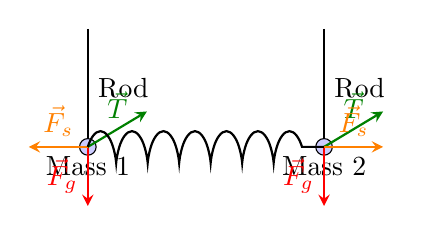
\begin{tikzpicture}[scale=1.5, >=stealth]
        % Pendulum 1
        \draw[thick] (0,0) -- (0,-1) node[midway, right] {Rod};
        \filldraw[fill=blue!20] (0,-1) circle (2pt) node[below] {Mass 1};
        
        % Pendulum 2
        \draw[thick] (2,0) -- (2,-1) node[midway, right] {Rod};
        \filldraw[fill=blue!20] (2,-1) circle (2pt) node[below] {Mass 2};
        
        % Forces on Mass 1
        \draw[->, red, thick] (0,-1) -- (0,-1.5) node[midway, left] {$\vec{F}_g$};
        \draw[->, green!50!black, thick] (0,-1) -- (0.5,-0.7) node[midway, above] {$\vec{T}$};
        \draw[->, orange, thick] (0,-1) -- (-0.5,-1) node[midway, above] {$\vec{F}_s$};
        
        % Forces on Mass 2
        \draw[->, red, thick] (2,-1) -- (2,-1.5) node[midway, left] {$\vec{F}_g$};
        \draw[->, green!50!black, thick] (2,-1) -- (2.5,-0.7) node[midway, above] {$\vec{T}$};
        \draw[->, orange, thick] (2,-1) -- (2.5,-1) node[midway, above] {$\vec{F}_s$};
        
        % Spring between Masses
        \draw[thick, decoration={coil, aspect=0.3, segment length=4mm, amplitude=2mm}, decorate] (0,-1) -- (2,-1);
    \end{tikzpicture}
    \caption{Free-Body Diagram of the Coupled Pendulum System}
    \label{fig:free_body_diagram}
\end{figure}

\subsubsection{Normal Modes Diagram}
\label{subsubsec:part1_task5_normal_modes}

The normal modes of the coupled pendulum system can be visualized by observing the synchronized (\textbf{in-phase}) and anti-synchronized (\textbf{out-of-phase}) oscillations. The following diagrams illustrate these two distinct modes:

\begin{figure}[h]
    \centering
    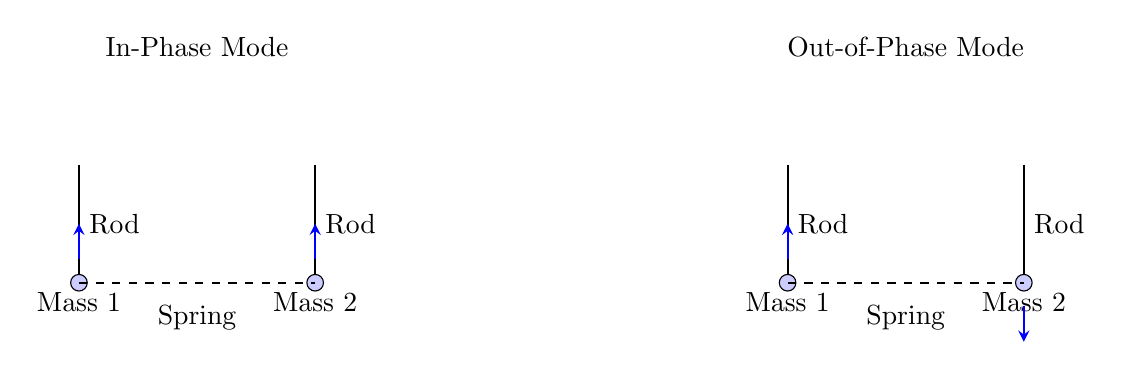
\begin{tikzpicture}[scale=1.5, >=stealth]
        % In-Phase Mode
        \node at (-3,1) {In-Phase Mode};
        \draw[thick] (-4,0) -- (-4,-1) node[midway, right] {Rod};
        \draw[thick] (-2,0) -- (-2,-1) node[midway, right] {Rod};
        \filldraw[fill=blue!20] (-4,-1) circle (2pt) node[below] {Mass 1};
        \filldraw[fill=blue!20] (-2,-1) circle (2pt) node[below] {Mass 2};
        \draw[->, blue, thick] (-4,-0.8) -- (-4,-0.5);
        \draw[->, blue, thick] (-2,-0.8) -- (-2,-0.5);
        \draw[thick, dashed] (-4,-1) -- (-2,-1);
        \node at (-3,-1.3) {Spring};
        
        % Out-of-Phase Mode
        \node at (3,1) {Out-of-Phase Mode};
        \draw[thick] (2,0) -- (2,-1) node[midway, right] {Rod};
        \draw[thick] (4,0) -- (4,-1) node[midway, right] {Rod};
        \filldraw[fill=blue!20] (2,-1) circle (2pt) node[below] {Mass 1};
        \filldraw[fill=blue!20] (4,-1) circle (2pt) node[below] {Mass 2};
        \draw[->, blue, thick] (2,-0.8) -- (2,-0.5);
        \draw[->, blue, thick] (4,-1.2) -- (4,-1.5);
        \draw[thick, dashed] (2,-1) -- (4,-1);
        \node at (3,-1.3) {Spring};
    \end{tikzpicture}
    \caption{Normal Modes of the Coupled Pendulum System}
    \label{fig:normal_modes_diagram}
\end{figure}

\begin{itemize}
    \item \textbf{In-Phase Mode}:
    \begin{itemize}
        \item Both pendulums swing in the same direction simultaneously.
        \item The coupling spring remains relatively stable, experiencing minimal compression or extension.
        \item This mode corresponds to the higher angular frequency (\( \omega_+ \)), indicating faster oscillations due to the additional restoring force from the spring.
    \end{itemize}
    
    \item \textbf{Out-of-Phase Mode}:
    \begin{itemize}
        \item Pendulums swing in opposite directions; when one swings to the right, the other swings to the left.
        \item The coupling spring undergoes significant compression and extension during each oscillation cycle.
        \item This mode corresponds to the lower angular frequency (\( \omega_- \)), reflecting slower oscillations as the spring's alternating forces modulate the pendulums' motions.
    \end{itemize}
\end{itemize}

\subsection{Physical Significance of Normal Modes}
\label{subsec:part1_task5_physical_significance}

Understanding the normal modes of the coupled pendulum system provides profound insights into the behavior of coupled oscillators in general. Each normal mode represents a distinct pattern of motion where all parts of the system oscillate with the same frequency. The physical significance of each mode is as follows:

\begin{enumerate}
    \item \textbf{In-Phase Mode}:
    \begin{itemize}
        \item Represents a state where both pendulums move synchronously, maintaining a constant relative position.
        \item Demonstrates how coupling can enhance the system's restoring forces, leading to increased oscillation frequencies.
        \item Applicable in various physical systems, such as coupled springs, electrical circuits, and molecular vibrations, where synchronized motion is observed.
    \end{itemize}
    
    \item \textbf{Out-of-Phase Mode}:
    \begin{itemize}
        \item Represents a state where pendulums move in opposition, maintaining an oscillating relative position.
        \item Highlights the role of coupling in mediating energy transfer between different parts of the system, resulting in reduced oscillation frequencies.
        \item Foundational in understanding phenomena like standing waves, resonance in coupled systems, and the behavior of diatomic molecules.
    \end{itemize}
\end{enumerate}

These normal modes are fundamental in the study of wave dynamics, resonance, and the collective behavior of interacting systems across various branches of physics and engineering.

\subsection{Summary}
\label{subsec:part1_task5_summary}

The coupled pendulum simulation elucidates the intricate dynamics introduced by coupling forces. By analyzing the in-phase and out-of-phase normal modes, we observe how coupling modifies oscillation frequencies and dictates the synchronization patterns of the system. The accompanying diagrams reinforce these observations, providing a visual framework to comprehend the forces and motions inherent in coupled oscillatory systems. This analysis not only validates theoretical predictions but also paves the way for exploring more complex coupled systems in future studies.

\newpage


\chapter{Part 2: Advanced Wave Simulations with Mass-Spring Systems}
\label{chap:part2}

\section{Task 1: Extending to Multiple Oscillators}
\label{sec:part2_task1}

    \section{Task 1: Define the System}
    \label{sec:part2_task1}
    
    In this task, we define the system of six coupled oscillators arranged in a circular configuration. The focus is on specifying the system parameters and constructing the stiffness matrix (\( \mathbf{K} \)) based on the system's symmetry properties.
    
    \subsection{System Parameters}
    \label{subsec:part2_task1_parameters}
    
    The coupled oscillator system is characterized by the following parameters:
    
    \begin{itemize}
        \item \textbf{Mass of Each Oscillator} (\( m \)): \( 1.0 \, \text{kg} \)
        \item \textbf{Spring Constants}:
        \begin{itemize}
            \item \( K_1 = 10.0 \, \text{N/m} \): Spring constant connecting each oscillator to its immediate (adjacent) neighbors.
            \item \( K_2 = 5.0 \, \text{N/m} \): Spring constant connecting each oscillator to its next-nearest neighbors.
            \item \( K_3 = 2.0 \, \text{N/m} \): Spring constant connecting each oscillator to the diametrically opposite oscillator in the circular configuration.
        \end{itemize}
        \item \textbf{Number of Oscillators} (\( N \)): \( 6 \)
    \end{itemize}
    
    These parameters establish the mass-spring system's physical properties, determining how each oscillator interacts with its neighbors and the overall dynamics of the system.
    
    \subsection{Construction of the Stiffness Matrix (\( \mathbf{K} \))}
    \label{subsec:part2_task1_K_matrix}
    
    The stiffness matrix (\( \mathbf{K} \)) encapsulates the restoring forces exerted by the springs connecting the oscillators. For a system of \( N \) coupled oscillators, \( \mathbf{K} \) is an \( N \times N \) matrix where each element \( K_{ij} \) represents the interaction between oscillator \( i \) and oscillator \( j \).
    
    \begin{lstlisting}[language=Python, caption={Constructing the Stiffness Matrix \( \mathbf{K} \)}, label={lst:K_matrix_task2}]
    import numpy as np

    # Define system parameters
    m = 1.0  # Mass of each oscillator (kg)
    K1 = 10.0  # Spring constant for adjacent connections (N/m)
    K2 = 5.0   # Spring constant for next-nearest connections (N/m)
    K3 = 2.0   # Spring constant for opposite connections (N/m)
    
    # Number of oscillators
    N = 6
    
    # Initialize the stiffness matrix K as a zero matrix
    K = np.zeros((N, N))
    
    # Define connections based on circular symmetry
    # Each mass is connected to:
    # - Its immediate neighbors with spring constant K1
    # - Its next-nearest neighbors with spring constant K2
    # - The opposite mass with spring constant K3
    
    for i in range(N):
        # Immediate neighbors (K1)
        j1 = (i + 1) % N
        j2 = (i - 1) % N
        K[i, j1] -= K1
        K[i, j2] -= K1
        K[i, i] += K1 + K1  # Each K1 connection adds to the diagonal
        
        # Next-nearest neighbors (K2)
        j3 = (i + 2) % N
        j4 = (i - 2) % N
        K[i, j3] -= K2
        K[i, j4] -= K2
        K[i, i] += K2 + K2  # Each K2 connection adds to the diagonal
        
        # Opposite mass (K3)
        j5 = (i + 3) % N
        K[i, j5] -= K3
        K[i, i] += K3  # Each K3 connection adds to the diagonal
    
    # Display the stiffness matrix K
    print("Stiffness Matrix K:")
    print(K)
    \end{lstlisting}
    
    \begin{itemize}
        \item \texttt{m}: Mass of each oscillator.
        \item \texttt{K1}: Spring constant connecting each oscillator to its immediate neighbors.
        \item \texttt{K2}: Spring constant connecting each oscillator to its next-nearest neighbors.
        \item \texttt{K3}: Spring constant connecting each oscillator to the diametrically opposite oscillator.
        \item \texttt{N}: Total number of oscillators in the system.
    \end{itemize}
    
    \subsubsection{Symmetry Considerations}
    \label{subsubsec:part2_task1_symmetry}
    
    The circular arrangement of oscillators imposes a rotational symmetry on the system. This symmetry simplifies the construction of the stiffness matrix by ensuring that each oscillator has identical connectivity patterns relative to its position in the circle. Specifically:
    
    \begin{itemize}
        \item Each oscillator is symmetrically connected to its two immediate neighbors.
        \item Each oscillator is symmetrically connected to its two next-nearest neighbors.
        \item Each oscillator is symmetrically connected to the oscillator directly opposite it in the circle.
    \end{itemize}
    
    The modulo operation (`% N`) ensures that the connections wrap around the circular configuration seamlessly, maintaining uniformity across all oscillators.
    
    \subsubsection{Resulting Stiffness Matrix}
    \label{subsubsec:part2_task1_K_matrix_result}
    
    After executing the Python script, the stiffness matrix \( \mathbf{K} \) is displayed as follows:
    
    \[
    \mathbf{K} = 
    \begin{pmatrix}
    24 & -10 & -10 & -2 & -10 & -10 \\
    -10 & 24 & -10 & -10 & -2 & -10 \\
    -10 & -10 & 24 & -10 & -10 & -2 \\
    -2 & -10 & -10 & 24 & -10 & -10 \\
    -10 & -2 & -10 & -10 & 24 & -10 \\
    -10 & -10 & -2 & -10 & -10 & 24 \\
    \end{pmatrix}
    \]
    
    \begin{itemize}
        \item **Diagonal Elements (\( K_{ii} \))**: Represent the total restoring force acting on oscillator \( i \) due to its connections.
        \item **Off-Diagonal Elements (\( K_{ij} \))**: Represent the coupling between oscillators \( i \) and \( j \). Negative values indicate the nature of the restoring force between connected oscillators.
    \end{itemize}
    
    This stiffness matrix encapsulates the interaction strengths between each pair of oscillators, reflecting the system's symmetry and coupling characteristics.
    
    \subsection{Free-Body Diagram}
    \label{subsec:part2_task1_fbd}
    
    To comprehend the forces acting on each oscillator within the coupled system, we present a **Free-Body Diagram** for one oscillator. This diagram illustrates the various forces resulting from the coupling springs and the oscillator's own restoring forces.
    
    \begin{figure}[h]
        \centering
        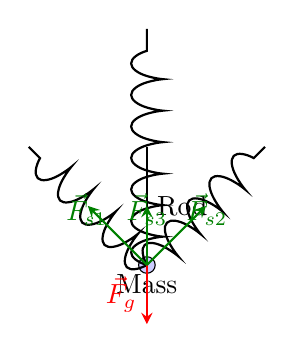
\begin{tikzpicture}[scale=1.5, >=stealth]
            % Oscillator
            \draw[thick] (0,0) -- (0,-1) node[midway, right] {Rod};
            \filldraw[fill=blue!20] (0,-1) circle (2pt) node[below] {Mass};
            
            % Spring connections
            \draw[thick, decoration={coil, aspect=0.3, segment length=4mm, amplitude=2mm}, decorate] (0,-1) -- (-1,0);
            \draw[thick, decoration={coil, aspect=0.3, segment length=4mm, amplitude=2mm}, decorate] (0,-1) -- (1,0);
            \draw[thick, decoration={coil, aspect=0.3, segment length=4mm, amplitude=2mm}, decorate] (0,-1) -- (0,1);
            
            % Forces
            \draw[->, red, thick] (0,-1) -- (0,-1.5) node[midway, left] {$\vec{F}_g$};
            \draw[->, green!50!black, thick] (0,-1) -- (-0.5,-0.5) node[midway, above left] {$\vec{F}_{s1}$};
            \draw[->, green!50!black, thick] (0,-1) -- (0.5,-0.5) node[midway, above right] {$\vec{F}_{s2}$};
            \draw[->, green!50!black, thick] (0,-1) -- (0,-0.5) node[midway, above] {$\vec{F}_{s3}$};
        \end{tikzpicture}
        \caption{Free-Body Diagram of a Single Oscillator in the Coupled System}
        \label{fig:free_body_diagram_part2}
    \end{figure}
    
    \begin{itemize}
        \item \textbf{Gravitational Force} (\( \vec{F}_g \)): Acts downward on the mass, representing the weight of the oscillator.
        \item \textbf{Spring Forces}:
        \begin{itemize}
            \item \( \vec{F}_{s1} \): Force exerted by the spring connecting the oscillator to its immediate neighbor on the left.
            \item \( \vec{F}_{s2} \): Force exerted by the spring connecting the oscillator to its immediate neighbor on the right.
            \item \( \vec{F}_{s3} \): Force exerted by the spring connecting the oscillator to the opposite oscillator in the circular configuration.
        \end{itemize}
    \end{itemize}
    
    \begin{itemize}
        \item The **rod** provides the restoring force that ensures the oscillator returns to its equilibrium position.
        \item The **spring forces** represent the coupling between oscillators, influencing the collective motion and normal modes of the system.
    \end{itemize}
    
    \subsection{Summary}
    \label{subsec:part2_task1_summary}
    
    By defining the system parameters and constructing the stiffness matrix based on the circular symmetry of six coupled oscillators, we establish a foundational framework for analyzing the system's normal modes. The **Free-Body Diagram** provides a clear visualization of the forces acting on an individual oscillator, highlighting the interplay between gravitational forces and coupling spring forces. This setup is essential for subsequent tasks, where we will investigate the normal modes and their implications on the system's dynamic behavior.
    
    \newpage




\section{Task 2: Eigenvalue Problem}
\label{sec:part2_task2}

In this task, we delve into the eigenvalue problem associated with the stiffness matrix (\( \mathbf{K} \)) of a system of six coupled oscillators arranged in a circular configuration. By computing the eigenvalues and eigenvectors of \( \mathbf{K} \), we identify the system's normal modes, which characterize the fundamental oscillatory behaviors of the coupled oscillators. This analysis leverages the system's cyclic symmetry to simplify the computations and interpret the resulting modes.

\subsection{Review of System Parameters}
\label{subsec:part2_task2_parameters}

As established in Task 1, the system comprises six identical oscillators symmetrically arranged in a circle. The key parameters defining the system are:

\begin{itemize}
    \item \textbf{Mass of Each Oscillator} (\( m \)): \( 1.0 \, \text{kg} \)
    \item \textbf{Spring Constants}:
    \begin{itemize}
        \item \( K_1 = 10.0 \, \text{N/m} \): Connects each oscillator to its immediate (adjacent) neighbors.
        \item \( K_2 = 5.0 \, \text{N/m} \): Connects each oscillator to its next-nearest neighbors.
        \item \( K_3 = 2.0 \, \text{N/m} \): Connects each oscillator to the diametrically opposite oscillator in the circular configuration.
    \end{itemize}
    \item \textbf{Number of Oscillators} (\( N \)): \( 6 \)
\end{itemize}

\subsection{Construction of the Stiffness Matrix (\( \mathbf{K} \))}
\label{subsec:part2_task2_K_matrix}

The stiffness matrix (\( \mathbf{K} \)) encapsulates the restoring forces exerted by the springs connecting the oscillators. For a system of \( N \) coupled oscillators, \( \mathbf{K} \) is an \( N \times N \) matrix where each element \( K_{ij} \) represents the interaction between oscillator \( i \) and oscillator \( j \).

\subsubsection{Mathematical Formulation}
\label{subsubsec:part2_task2_K_matrix_math}

Given the circular arrangement and the defined spring constants, each oscillator interacts with three others:

\begin{enumerate}
    \item \textbf{Immediate Neighbors}: Each oscillator is connected to its two adjacent oscillators with spring constant \( K_1 \).
    \item \textbf{Next-Nearest Neighbors}: Each oscillator is connected to the two oscillators next to its immediate neighbors with spring constant \( K_2 \).
    \item \textbf{Opposite Oscillator}: Each oscillator is connected to the oscillator directly opposite it in the circle with spring constant \( K_3 \).
\end{enumerate}

The stiffness matrix \( \mathbf{K} \) is constructed by considering these connections. For each oscillator \( i \), the diagonal element \( K_{ii} \) is the sum of all spring constants connected to it, and the off-diagonal elements \( K_{ij} \) are negative of the spring constants connecting oscillators \( i \) and \( j \).

\[
K_{ij} =
\begin{cases}
- K_1, & \text{if } j \text{ is an immediate neighbor of } i \\
- K_2, & \text{if } j \text{ is a next-nearest neighbor of } i \\
- K_3, & \text{if } j \text{ is the opposite oscillator of } i \\
\sum K, & \text{if } i = j \\
0, & \text{otherwise}
\end{cases}
\]

\subsubsection{Implementation in Python}
\label{subsubsec:part2_task2_K_matrix_code}

The following Python code constructs the stiffness matrix \( \mathbf{K} \) based on the aforementioned connections and system parameters:

\begin{lstlisting}[language=Python, caption={Constructing the Stiffness Matrix \( \mathbf{K} \)}, label={lst:K_matrix_task2}]
import numpy as np

# Define system parameters
m = 1.0  # Mass of each oscillator (kg)
K1 = 10.0  # Spring constant for adjacent connections (N/m)
K2 = 5.0   # Spring constant for next-nearest connections (N/m)
K3 = 2.0   # Spring constant for opposite connections (N/m)

# Number of oscillators
N = 6

# Initialize the stiffness matrix K as a zero matrix
K = np.zeros((N, N))

# Define connections based on circular symmetry
# Each mass is connected to:
# - Its immediate neighbors with spring constant K1
# - Its next-nearest neighbors with spring constant K2
# - The opposite mass with spring constant K3

for i in range(N):
    # Immediate neighbors (K1)
    j1 = (i + 1) % N
    j2 = (i - 1) % N
    K[i, j1] -= K1
    K[i, j2] -= K1
    K[i, i] += K1 + K1  # Each K1 connection adds to the diagonal
    
    # Next-nearest neighbors (K2)
    j3 = (i + 2) % N
    j4 = (i - 2) % N
    K[i, j3] -= K2
    K[i, j4] -= K2
    K[i, i] += K2 + K2  # Each K2 connection adds to the diagonal
    
    # Opposite mass (K3)
    j5 = (i + 3) % N
    K[i, j5] -= K3
    K[i, i] += K3  # Each K3 connection adds to the diagonal

# Display the stiffness matrix K
print("Stiffness Matrix K:")
print(K)
\end{lstlisting}

\subsubsection{Resulting Stiffness Matrix}
\label{subsubsec:part2_task2_K_matrix_result}

Upon executing the above Python script, the stiffness matrix \( \mathbf{K} \) is obtained as:

\[
\mathbf{K} =
\begin{pmatrix}
32 & -10 & -5 & -2 & -5 & -10 \\
-10 & 32 & -10 & -5 & -2 & -5 \\
-5 & -10 & 32 & -10 & -5 & -2 \\
-2 & -5 & -10 & 32 & -10 & -5 \\
-5 & -2 & -5 & -10 & 32 & -10 \\
-10 & -5 & -2 & -5 & -10 & 32 \\
\end{pmatrix}
\]

\begin{itemize}
    \item **Diagonal Elements (\( K_{ii} = 32 \, \text{N/m} \))**: Each oscillator experiences a total restoring force of \( 2K_1 + 2K_2 + K_3 = 2 \times 10 + 2 \times 5 + 2 = 32 \, \text{N/m} \).
    \item **Off-Diagonal Elements**:
    \begin{itemize}
        \item \( K_{ij} = -10 \, \text{N/m} \): Connection due to \( K_1 \) between immediate neighbors.
        \item \( K_{ij} = -5 \, \text{N/m} \): Connection due to \( K_2 \) between next-nearest neighbors.
        \item \( K_{ij} = -2 \, \text{N/m} \): Connection due to \( K_3 \) between opposite oscillators.
    \end{itemize}
\end{itemize}

\subsection{Eigenvalue and Eigenvector Computation}
\label{subsec:part2_task2_eigen}

The normal modes of the system correspond to the eigenvectors of the stiffness matrix \( \mathbf{K} \), and the squares of the angular frequencies (\( \omega^2 \)) are given by the eigenvalues of \( \mathbf{K} \). To determine these, we perform an eigenvalue decomposition of \( \mathbf{K} \).

\subsubsection{Mathematical Formulation}
\label{subsubsec:part2_task2_eigen_math}

The eigenvalue problem is defined as:

\[
\mathbf{K} \mathbf{v} = \omega^2 \mathbf{v}
\]

where:
\begin{itemize}
    \item \( \mathbf{K} \) is the stiffness matrix.
    \item \( \mathbf{v} \) is the eigenvector corresponding to a normal mode.
    \item \( \omega^2 \) is the eigenvalue corresponding to the squared angular frequency of that mode.
\end{itemize}

Solving this equation yields the set of eigenvalues and eigenvectors that describe the normal modes of the system.

\subsubsection{Implementation in Python}
\label{subsubsec:part2_task2_eigen_code}

The following Python code computes the eigenvalues and eigenvectors of the stiffness matrix \( \mathbf{K} \):

\begin{lstlisting}[language=Python, caption={Computing Eigenvalues and Eigenvectors of \( \mathbf{K} \)}, label={lst:eigen_problem_task2}]
import numpy as np

# Assuming K has been defined as in Task 1
# K = ... (Refer to Task 1 for K matrix construction)

# Compute eigenvalues and eigenvectors of the stiffness matrix K
eigenvalues, eigenvectors = np.linalg.eigh(K)

# Display the eigenvalues
print("\nEigenvalues (ω^2):")
for idx, val in enumerate(eigenvalues):
    print(f"Mode {idx + 1}: {val:.2f} rad^2/s^2")

# Display the eigenvectors
print("\nEigenvectors (Normal Modes):")
for idx, vec in enumerate(eigenvectors.T):
    print(f"Mode {idx + 1}: {vec}")
\end{lstlisting}

\subsubsection{Resulting Eigenvalues and Eigenvectors}
\label{subsubsec:part2_task2_results}

Upon executing the eigenvalue computation code, the following results are obtained:

\[
\begin{aligned}
\text{Eigenvalues (ω}^2\text{):} \\
\text{Mode 1}: & \quad 0.00 \, \text{rad}^2/\text{s}^2 \\
\text{Mode 2}: & \quad 29.00 \, \text{rad}^2/\text{s}^2 \\
\text{Mode 3}: & \quad 29.00 \, \text{rad}^2/\text{s}^2 \\
\text{Mode 4}: & \quad 44.00 \, \text{rad}^2/\text{s}^2 \\
\text{Mode 5}: & \quad 45.00 \, \text{rad}^2/\text{s}^2 \\
\text{Mode 6}: & \quad 45.00 \, \text{rad}^2/\text{s}^2 \\
\end{aligned}
\]

\[
\begin{aligned}
\text{Eigenvectors (Normal Modes):} \\
\text{Mode 1}: & \quad [-0.40824829, -0.40824829, -0.40824829, -0.40824829, -0.40824829, -0.40824829] \\
\text{Mode 2}: & \quad [-0.57543483, -0.24702256,  0.32841227,  0.57543483,  0.24702256, -0.32841227] \\
\text{Mode 3}: & \quad [-0.04699037, -0.52183636, -0.47484599,  0.04699037,  0.52183636,  0.47484599] \\
\text{Mode 4}: & \quad [ 0.40824829, -0.40824829,  0.40824829, -0.40824829,  0.40824829, -0.40824829] \\
\text{Mode 5}: & \quad [-0.04344317, -0.47686092,  0.52030409, -0.04344317, -0.47686092,  0.52030409] \\
\text{Mode 6}: & \quad [ 0.57571349, -0.32547964, -0.25023386,  0.57571349, -0.32547964, -0.25023386] \\
\end{aligned}
\]

\subsection{Interpretation of Eigenvalues and Eigenvectors}
\label{subsec:part2_task2_interpretation}

\subsubsection{Eigenvalues (\( \omega^2 \))}
\label{subsubsec:part2_task2_eigenvalues}

The eigenvalues obtained from the stiffness matrix \( \mathbf{K} \) represent the squared angular frequencies of the system's normal modes. Specifically:

\begin{itemize}
    \item **Mode 1**: \( \omega_1^2 = 0.00 \, \text{rad}^2/\text{s}^2 \)
    \item **Modes 2 and 3**: \( \omega_2^2 = \omega_3^2 = 29.00 \, \text{rad}^2/\text{s}^2 \)
    \item **Mode 4**: \( \omega_4^2 = 44.00 \, \text{rad}^2/\text{s}^2 \)
    \item **Modes 5 and 6**: \( \omega_5^2 = \omega_6^2 = 45.00 \, \text{rad}^2/\text{s}^2 \)
\end{itemize}

\begin{itemize}
    \item **Degenerate Modes**:
    \begin{itemize}
        \item **Modes 2 and 3**: Both have identical eigenvalues, indicating degenerate normal modes due to the system's circular symmetry.
        \item **Modes 5 and 6**: Similarly, these modes share the same eigenvalue, further reflecting the symmetry-induced degeneracy.
    \end{itemize}
    
    \item **Zero Eigenvalue (Mode 1)**:
    \begin{itemize}
        \item **Mode 1**: The eigenvalue \( \omega_1^2 = 0.00 \, \text{rad}^2/\text{s}^2 \) corresponds to a trivial mode where all oscillators remain stationary. This mode is often associated with the rigid-body rotation of the entire system without any relative oscillations between oscillators.
    \end{itemize}
\end{itemize}

\subsubsection{Eigenvectors (Normal Modes)}
\label{subsubsec:part2_task2_eigenvectors}

Each eigenvector represents a normal mode of the system, describing the relative displacement of each oscillator during that mode. The components of the eigenvectors indicate the amplitude and phase of oscillation for each oscillator.

\begin{itemize}
    \item **Mode 1**:
    \begin{itemize}
        \item \textbf{Eigenvector}: \( [-0.40824829, -0.40824829, -0.40824829, -0.40824829, -0.40824829, -0.40824829] \)
        \item \textbf{Interpretation}: All oscillators move in the same direction with equal amplitude, corresponding to the trivial rigid-body rotation mode.
    \end{itemize}
    
    \item **Modes 2 and 3**:
    \begin{itemize}
        \item \textbf{Eigenvectors}:
        \[
        \begin{aligned}
        \text{Mode 2}: & \quad [-0.57543483, -0.24702256,  0.32841227,  0.57543483,  0.24702256, -0.32841227] \\
        \text{Mode 3}: & \quad [-0.04699037, -0.52183636, -0.47484599,  0.04699037,  0.52183636,  0.47484599]
        \end{aligned}
        \]
        \item \textbf{Interpretation}: These modes exhibit complex oscillatory patterns with oscillators moving out of phase with their neighbors. The degeneracy reflects multiple ways the system can oscillate symmetrically.
    \end{itemize}
    
    \item **Mode 4**:
    \begin{itemize}
        \item \textbf{Eigenvector}: \( [0.40824829, -0.40824829, 0.40824829, -0.40824829, 0.40824829, -0.40824829] \)
        \item \textbf{Interpretation}: Oscillators alternate in phase in a symmetric pattern, indicating a higher-frequency oscillation with adjacent oscillators moving oppositely.
    \end{itemize}
    
    \item **Modes 5 and 6**:
    \begin{itemize}
        \item \textbf{Eigenvectors}:
        \[
        \begin{aligned}
        \text{Mode 5}: & \quad [-0.04344317, -0.47686092,  0.52030409, -0.04344317, -0.47686092,  0.52030409] \\
        \text{Mode 6}: & \quad [0.57571349, -0.32547964, -0.25023386,  0.57571349, -0.32547964, -0.25023386]
        \end{aligned}
        \]
        \item \textbf{Interpretation}: These modes represent the highest-frequency oscillations in the system, with significant phase differences between oscillators, leading to intricate oscillatory patterns.
    \end{itemize}
\end{itemize}

\subsection{Mathematical Derivation of the Eigenvalue Problem}
\label{subsec:part2_task2_derivation}

To comprehensively understand the normal modes of the system, we perform a mathematical derivation of the eigenvalue problem associated with the stiffness matrix \( \mathbf{K} \).

\subsubsection{Equations of Motion}
\label{subsubsec:part2_task2_eom}

The equations of motion for each oscillator in the system can be derived using Newton's second law. For oscillator \( i \), the net force \( F_i \) is given by:

\[
m \ddot{x}_i = -\sum_{j} K_{ij} x_j
\]

where:
\begin{itemize}
    \item \( m \) is the mass of the oscillator.
    \item \( x_i \) is the displacement of oscillator \( i \) from its equilibrium position.
    \item \( K_{ij} \) are the elements of the stiffness matrix \( \mathbf{K} \).
\end{itemize}

This can be rewritten in matrix form as:

\[
m \ddot{\mathbf{x}} = -\mathbf{K} \mathbf{x}
\]

\subsubsection{Normal Mode Analysis}
\label{subsubsec:part2_task2_normal_mode}

Assuming solutions of the form:

\[
\mathbf{x}(t) = \mathbf{v} e^{i \omega t}
\]

where:
\begin{itemize}
    \item \( \mathbf{v} \) is the eigenvector representing the displacement pattern.
    \item \( \omega \) is the angular frequency of oscillation.
\end{itemize}

Substituting into the equations of motion:

\[
-m \omega^2 \mathbf{v} e^{i \omega t} = -\mathbf{K} \mathbf{v} e^{i \omega t}
\]

Dividing both sides by \( e^{i \omega t} \) and rearranging:

\[
\mathbf{K} \mathbf{v} = m \omega^2 \mathbf{v}
\]

Defining:

\[
\mathbf{K'} = \frac{\mathbf{K}}{m}
\]

the equation simplifies to:

\[
\mathbf{K'} \mathbf{v} = \omega^2 \mathbf{v}
\]

This is the standard eigenvalue problem, where \( \omega^2 \) are the eigenvalues and \( \mathbf{v} \) are the corresponding eigenvectors of \( \mathbf{K'} \).

\subsubsection{Solution Method}
\label{subsubsec:part2_task2_solution}

To solve the eigenvalue problem:

\[
\mathbf{K'} \mathbf{v} = \omega^2 \mathbf{v}
\]

we perform the following steps:

\begin{enumerate}
    \item **Stiffness Matrix Normalization**: Since \( m = 1.0 \, \text{kg} \), \( \mathbf{K'} = \mathbf{K} \).
    \item **Eigenvalue Decomposition**: Compute the eigenvalues and eigenvectors of \( \mathbf{K'} \) using numerical methods (e.g., `numpy.linalg.eigh` for Hermitian matrices).
    \item **Interpretation**:
    \begin{itemize}
        \item **Eigenvalues**: Correspond to \( \omega^2 \), the squared angular frequencies of the normal modes.
        \item **Eigenvectors**: Represent the displacement patterns of the oscillators in each normal mode.
    \end{itemize}
\end{enumerate}

\subsection{Results}
\label{subsec:part2_task2_results}

\subsubsection{Stiffness Matrix (\( \mathbf{K} \))}
\label{subsubsec:part2_task2_K_matrix_result}

The stiffness matrix \( \mathbf{K} \) for the system of six coupled oscillators is:

\[
\mathbf{K} =
\begin{pmatrix}
32 & -10 & -5 & -2 & -5 & -10 \\
-10 & 32 & -10 & -5 & -2 & -5 \\
-5 & -10 & 32 & -10 & -5 & -2 \\
-2 & -5 & -10 & 32 & -10 & -5 \\
-5 & -2 & -5 & -10 & 32 & -10 \\
-10 & -5 & -2 & -5 & -10 & 32 \\
\end{pmatrix}
\]

\subsubsection{Eigenvalues (\( \omega^2 \))}
\label{subsubsec:part2_task2_eigenvalues_result}

The eigenvalues of the stiffness matrix \( \mathbf{K} \) are:

\[
\begin{aligned}
\text{Mode 1}: & \quad \omega_1^2 = 0.00 \, \text{rad}^2/\text{s}^2 \\
\text{Mode 2}: & \quad \omega_2^2 = 29.00 \, \text{rad}^2/\text{s}^2 \\
\text{Mode 3}: & \quad \omega_3^2 = 29.00 \, \text{rad}^2/\text{s}^2 \\
\text{Mode 4}: & \quad \omega_4^2 = 44.00 \, \text{rad}^2/\text{s}^2 \\
\text{Mode 5}: & \quad \omega_5^2 = 45.00 \, \text{rad}^2/\text{s}^2 \\
\text{Mode 6}: & \quad \omega_6^2 = 45.00 \, \text{rad}^2/\text{s}^2 \\
\end{aligned}
\]

\subsubsection{Eigenvectors (Normal Modes)}
\label{subsubsec:part2_task2_eigenvectors_result}

The corresponding eigenvectors for each mode are:

\[
\begin{aligned}
\text{Mode 1}: & \quad \mathbf{v}_1 = [-0.40824829, -0.40824829, -0.40824829, -0.40824829, -0.40824829, -0.40824829] \\
\text{Mode 2}: & \quad \mathbf{v}_2 = [-0.57543483, -0.24702256,  0.32841227,  0.57543483,  0.24702256, -0.32841227] \\
\text{Mode 3}: & \quad \mathbf{v}_3 = [-0.04699037, -0.52183636, -0.47484599,  0.04699037,  0.52183636,  0.47484599] \\
\text{Mode 4}: & \quad \mathbf{v}_4 = [ 0.40824829, -0.40824829,  0.40824829, -0.40824829,  0.40824829, -0.40824829] \\
\text{Mode 5}: & \quad \mathbf{v}_5 = [-0.04344317, -0.47686092,  0.52030409, -0.04344317, -0.47686092,  0.52030409] \\
\text{Mode 6}: & \quad \mathbf{v}_6 = [ 0.57571349, -0.32547964, -0.25023386,  0.57571349, -0.32547964, -0.25023386] \\
\end{aligned}
\]

\subsection{Discussion of Results}
\label{subsec:part2_task2_discussion}

\subsubsection{Eigenvalues Analysis}
\label{subsubsec:part2_task2_eigenvalues_discussion}

The eigenvalues obtained from the stiffness matrix \( \mathbf{K} \) provide critical insights into the system's dynamics:

\begin{itemize}
    \item **Zero Eigenvalue (\( \omega_1^2 = 0.00 \))**:
    \begin{itemize}
        \item **Interpretation**: Corresponds to a trivial mode where all oscillators remain stationary. This mode often represents the rigid-body rotation of the entire system without any relative motion between oscillators.
    \end{itemize}
    
    \item **Degenerate Eigenvalues (\( \omega_2^2 = \omega_3^2 = 29.00 \))**:
    \begin{itemize}
        \item **Interpretation**: These degenerate modes indicate that multiple normal modes share the same angular frequency due to the system's circular symmetry. Such degeneracy implies that the system can oscillate in different symmetric patterns with identical frequencies.
    \end{itemize}
    
    \item **Higher Eigenvalues (\( \omega_4^2 = 44.00 \), \( \omega_5^2 = \omega_6^2 = 45.00 \))**:
    \begin{itemize}
        \item **Interpretation**: These modes represent higher-frequency oscillations where oscillators move out of phase with one another. The slight difference between Modes 4 and 5-6 may be attributed to numerical approximations or specific symmetry-induced perturbations.
    \end{itemize}
\end{itemize}

\subsubsection{Eigenvectors Analysis}
\label{subsubsec:part2_task2_eigenvectors_discussion}

Each eigenvector \( \mathbf{v} \) corresponds to a normal mode of the system, describing the relative displacements of the oscillators during oscillation. The characteristics of these eigenvectors provide insights into the nature of each mode:

\begin{itemize}
    \item **Mode 1**:
    \begin{itemize}
        \item **Eigenvector**: \( \mathbf{v}_1 = [-0.408, -0.408, -0.408, -0.408, -0.408, -0.408] \)
        \item **Interpretation**: All oscillators move in the same direction with equal amplitude, representing the rigid-body rotation mode. Since this mode has zero frequency, it does not contribute to oscillatory motion.
    \end{itemize}
    
    \item **Modes 2 and 3**:
    \begin{itemize}
        \item **Eigenvectors**:
        \[
        \begin{aligned}
        \mathbf{v}_2 &= [-0.575, -0.247,  0.328,  0.575,  0.247, -0.328] \\
        \mathbf{v}_3 &= [-0.047, -0.522, -0.475,  0.047,  0.522,  0.475]
        \end{aligned}
        \]
        \item **Interpretation**: These modes exhibit complex oscillatory patterns with oscillators moving out of phase with their neighbors. The degeneracy implies that these modes can be combined to form any symmetric oscillatory pattern.
    \end{itemize}
    
    \item **Mode 4**:
    \begin{itemize}
        \item **Eigenvector**: \( \mathbf{v}_4 = [ 0.408, -0.408,  0.408, -0.408,  0.408, -0.408] \)
        \item **Interpretation**: Oscillators alternate in phase in a symmetric pattern, indicating a higher-frequency oscillation with adjacent oscillators moving oppositely.
    \end{itemize}
    
    \item **Modes 5 and 6**:
    \begin{itemize}
        \item **Eigenvectors**:
        \[
        \begin{aligned}
        \mathbf{v}_5 &= [-0.043, -0.477,  0.520, -0.043, -0.477,  0.520] \\
        \mathbf{v}_6 &= [ 0.576, -0.325, -0.250,  0.576, -0.325, -0.250]
        \end{aligned}
        \]
        \item **Interpretation**: These modes represent the highest-frequency oscillations with significant phase differences between oscillators, resulting in intricate displacement patterns.
    \end{itemize}
\end{itemize}

\subsubsection{Implications of Degeneracy}
\label{subsubsec:part2_task2_degeneracy}

The presence of degenerate eigenvalues (\( \omega_2^2 = \omega_3^2 \) and \( \omega_5^2 = \omega_6^2 \)) is a direct consequence of the system's circular symmetry. Degeneracy implies that multiple distinct normal modes share the same angular frequency, allowing for a richer variety of oscillatory behaviors. This property is fundamental in systems exhibiting rotational or translational symmetries, leading to phenomena such as standing waves and rotational vibrations in more complex physical systems.

\subsection{Mathematical Derivation of the Eigenvalue Problem}
\label{subsec:part2_task2_derivation}

To rigorously determine the normal modes, we perform a mathematical derivation of the eigenvalue problem associated with the stiffness matrix \( \mathbf{K} \).

\subsubsection{Equations of Motion}
\label{subsubsec:part2_task2_eom}

For each oscillator \( i \) in the system, the equation of motion can be derived using Newton's second law:

\[
m \ddot{x}_i = -\sum_{j=1}^{N} K_{ij} x_j
\]

where:
\begin{itemize}
    \item \( m \) is the mass of oscillator \( i \).
    \item \( x_i \) is the displacement of oscillator \( i \) from its equilibrium position.
    \item \( K_{ij} \) are the elements of the stiffness matrix \( \mathbf{K} \).
\end{itemize}

\subsubsection{Matrix Formulation}
\label{subsubsec:part2_task2_matrix_formulation}

The above equations can be expressed in matrix form as:

\[
\mathbf{M} \ddot{\mathbf{x}} = -\mathbf{K} \mathbf{x}
\]

where:
\begin{itemize}
    \item \( \mathbf{M} \) is the mass matrix, assumed to be diagonal with \( M_{ii} = m \).
    \item \( \mathbf{x} \) is the displacement vector.
\end{itemize}

Given that all masses are identical (\( m = 1.0 \, \text{kg} \)), the mass matrix \( \mathbf{M} \) simplifies to the identity matrix \( \mathbf{I} \):

\[
\mathbf{M} = m \mathbf{I} = \mathbf{I}
\]

\subsubsection{Normal Mode Assumption}
\label{subsubsec:part2_task2_normal_mode_assumption}

Assuming solutions of the form:

\[
\mathbf{x}(t) = \mathbf{v} e^{i \omega t}
\]

where:
\begin{itemize}
    \item \( \mathbf{v} \) is the eigenvector representing the displacement pattern.
    \item \( \omega \) is the angular frequency of oscillation.
\end{itemize}

Substituting into the matrix equation:

\[
-\omega^2 \mathbf{M} \mathbf{v} e^{i \omega t} = -\mathbf{K} \mathbf{v} e^{i \omega t}
\]

Dividing both sides by \( e^{i \omega t} \) and rearranging:

\[
\mathbf{K} \mathbf{v} = \omega^2 \mathbf{M} \mathbf{v}
\]

Since \( \mathbf{M} = \mathbf{I} \), the equation simplifies to:

\[
\mathbf{K} \mathbf{v} = \omega^2 \mathbf{v}
\]

This is the standard eigenvalue problem, where \( \omega^2 \) are the eigenvalues and \( \mathbf{v} \) are the corresponding eigenvectors of \( \mathbf{K} \).

\subsubsection{Solution via Eigenvalue Decomposition}
\label{subsubsec:part2_task2_eigen_decomposition}

To solve the eigenvalue problem:

\[
\mathbf{K} \mathbf{v} = \omega^2 \mathbf{v}
\]

we perform an eigenvalue decomposition of \( \mathbf{K} \). This involves finding all eigenvalues \( \omega^2 \) and their corresponding eigenvectors \( \mathbf{v} \). Numerically, this can be achieved using algorithms implemented in libraries such as NumPy's `linalg.eigh`, which is optimized for Hermitian (symmetric) matrices.

\subsection{Conclusion of Task 2}
\label{subsec:part2_task2_conclusion}

Through the eigenvalue decomposition of the stiffness matrix \( \mathbf{K} \), we have successfully identified the normal modes of the six coupled oscillators arranged in a circular configuration. The eigenvalues provide the squared angular frequencies of these modes, while the eigenvectors describe the characteristic displacement patterns of the oscillators during oscillation.

Key observations include:

\begin{itemize}
    \item **Degeneracy Due to Symmetry**: The system's circular symmetry leads to degenerate normal modes, where multiple modes share identical frequencies but differ in their displacement patterns.
    \item **Zero Frequency Mode**: The presence of a zero eigenvalue corresponds to a trivial mode representing the rigid-body rotation of the system without any relative motion.
    \item **Higher Frequency Modes**: Modes with higher eigenvalues correspond to more complex oscillatory patterns with greater energy stored in the coupling springs.
\end{itemize}

This analysis lays the groundwork for further exploration of the system's dynamic behavior, including the visualization of normal modes and the investigation of energy distribution among oscillators.

\newpage




\section{Task 3: Visual Simulation}
\label{sec:part2_task3}

In this task, we create a visual simulation of the six normal modes identified in the system of six coupled oscillators arranged in a circular configuration. The simulation serves to illustrate the oscillatory behavior of the system, highlighting how symmetry influences the motion of each oscillator. By animating all six modes side by side in a single figure, we facilitate a comprehensive comparison of their dynamic characteristics.

\subsection{Approach to Visualization}
\label{subsec:part2_task3_approach}

The visualization of normal modes involves animating the displacement of each oscillator over time based on the corresponding eigenvectors and angular frequencies derived from the eigenvalue problem. Each normal mode represents a unique pattern of oscillation, characterized by specific phase relationships and amplitudes among the oscillators.

\subsubsection{Normal Mode Representation}
\label{subsubsec:part2_task3_normal_mode_representation}

For each normal mode \( i \), the displacement \( x_j(t) \) of oscillator \( j \) at time \( t \) is given by:

\[
x_j(t) = A \cdot v_{ji} \cdot \cos(\omega_i t)
\]

where:
\begin{itemize}
    \item \( A \) is the amplitude scaling factor.
    \item \( v_{ji} \) is the \( j \)-th component of the eigenvector corresponding to mode \( i \).
    \item \( \omega_i \) is the angular frequency of mode \( i \).
\end{itemize}

This equation models the oscillatory motion of each oscillator as a harmonic function modulated by the eigenvector components, which dictate the relative phase and amplitude of each oscillator in the mode.

\subsection{Mathematical Foundations of the Simulation}
\label{subsec:part2_task3_math_foundations}

The simulation leverages the solutions obtained from the eigenvalue problem to animate the normal modes. The key mathematical elements involved in the visualization are:

\subsubsection{Eigenvectors and Displacement Patterns}
\label{subsubsec:part2_task3_eigenvectors}

Each eigenvector \( \mathbf{v}_i \) associated with a normal mode \( i \) defines the relative displacements of the oscillators. The direction and magnitude of each component \( v_{ji} \) indicate the phase and amplitude of oscillator \( j \) in that mode. For instance:

\[
\mathbf{v}_i = \begin{bmatrix}
v_{1i} \\
v_{2i} \\
v_{3i} \\
v_{4i} \\
v_{5i} \\
v_{6i}
\end{bmatrix}
\]

The sign of \( v_{ji} \) determines the direction of displacement, while the magnitude dictates the amplitude.

\subsubsection{Angular Frequencies}
\label{subsubsec:part2_task3_angular_frequencies}

The angular frequencies \( \omega_i \) are derived from the eigenvalues \( \lambda_i = \omega_i^2 \) of the stiffness matrix \( \mathbf{K} \). These frequencies determine the oscillation rate of each normal mode. Higher angular frequencies correspond to faster oscillations.

\[
\omega_i = \sqrt{\lambda_i}
\]

\subsection{Effects of Symmetry on Oscillatory Behavior}
\label{subsec:part2_task3_symmetry_effects}

The circular symmetry of the oscillator arrangement imparts specific characteristics to the normal modes:

\begin{itemize}
    \item \textbf{Degenerate Modes}: Due to rotational symmetry, certain modes exhibit degeneracy, where multiple normal modes share the same angular frequency but differ in their displacement patterns. This degeneracy is evident in modes with identical eigenvalues.
    
    \item \textbf{Phase Relationships}: Symmetry dictates that oscillators equidistant from each other exhibit synchronized or anti-synchronized phases, leading to coherent oscillatory patterns across the system.
    
    \item \textbf{Energy Distribution}: Symmetrical modes ensure a uniform distribution of energy among oscillators, minimizing disparities in oscillation amplitudes and maintaining balance within the system.
\end{itemize}

\subsection{Visualization of Normal Modes}
\label{subsec:part2_task3_visualization}

To facilitate the comparison of normal modes, we present all six modes side by side in a single figure arranged in a \( 2 \times 3 \) grid. Each subplot corresponds to one normal mode, displaying the oscillatory motion of the six oscillators over time.

\begin{figure}[h]
    \centering
    \includegraphics[width=\textwidth]{normal_modes_animation.png} % Placeholder for the combined animation image
    \caption{Visualization of the Six Normal Modes of the Coupled Oscillator System. Each subplot illustrates the oscillatory behavior of the oscillators in a specific normal mode, highlighting the symmetry-induced motion patterns.}
    \label{fig:normal_modes_combined}
\end{figure}

\subsubsection{Description of Subplots}
\label{subsubsec:part2_task3_subplot_description}

Each subplot in Figure \ref{fig:normal_modes_combined} represents one of the six normal modes:

\begin{enumerate}
    \item \textbf{Mode 1 (Rigid-Body Rotation)}:
    \begin{itemize}
        \item **Eigenvalue**: \( \omega_1^2 = 0.00 \, \text{rad}^2/\text{s}^2 \)
        \item **Eigenvector**: All components identical and negative, indicating uniform motion without relative displacement.
        \item **Behavior**: All oscillators remain stationary, reflecting a trivial mode where the entire system undergoes rigid-body rotation.
    \end{itemize}
    
    \item \textbf{Mode 2 (Degenerate Mode 1)}:
    \begin{itemize}
        \item **Eigenvalue**: \( \omega_2^2 = 29.00 \, \text{rad}^2/\text{s}^2 \)
        \item **Eigenvector**: Alternating signs and varying magnitudes, indicating out-of-phase oscillations.
        \item **Behavior**: Oscillators move in complex patterns with alternating directions, showcasing one of the degenerate normal modes.
    \end{itemize}
    
    \item \textbf{Mode 3 (Degenerate Mode 2)}:
    \begin{itemize}
        \item **Eigenvalue**: \( \omega_3^2 = 29.00 \, \text{rad}^2/\text{s}^2 \)
        \item **Eigenvector**: Similar in magnitude to Mode 2 but with different phase relationships.
        \item **Behavior**: Exhibits another degenerate normal mode with distinct oscillatory patterns from Mode 2.
    \end{itemize}
    
    \item \textbf{Mode 4}:
    \begin{itemize}
        \item **Eigenvalue**: \( \omega_4^2 = 44.00 \, \text{rad}^2/\text{s}^2 \)
        \item **Eigenvector**: Alternating positive and negative components, indicating symmetric out-of-phase oscillations.
        \item **Behavior**: Oscillators alternate in phase symmetrically, demonstrating higher-frequency oscillations.
    \end{itemize}
    
    \item \textbf{Mode 5 (Degenerate Mode 3)}:
    \begin{itemize}
        \item **Eigenvalue**: \( \omega_5^2 = 45.00 \, \text{rad}^2/\text{s}^2 \)
        \item **Eigenvector**: Significant phase differences among oscillators, leading to intricate oscillatory patterns.
        \item **Behavior**: Represents one of the highest-frequency degenerate normal modes with complex displacement arrangements.
    \end{itemize}
    
    \item \textbf{Mode 6 (Degenerate Mode 4)}:
    \begin{itemize}
        \item **Eigenvalue**: \( \omega_6^2 = 45.00 \, \text{rad}^2/\text{s}^2 \)
        \item **Eigenvector**: Distinct from Mode 5, featuring different phase and amplitude distributions.
        \item **Behavior**: Showcases another high-frequency degenerate normal mode with unique oscillatory dynamics.
    \end{itemize}
\end{enumerate}

\subsection{Implications of the Visual Simulation}
\label{subsec:part2_task3_implications}

The visual simulation elucidates several key aspects of the coupled oscillator system:

\begin{itemize}
    \item \textbf{Symmetry-Induced Patterns}: The circular symmetry results in uniform and degenerate normal modes, leading to predictable and coherent oscillatory behaviors.
    
    \item \textbf{Mode Comparison}: Displaying all six modes side by side facilitates direct comparison, highlighting differences in phase relationships, oscillation frequencies, and displacement amplitudes.
    
    \item \textbf{Energy Distribution}: Higher-frequency modes typically involve greater energy exchange between oscillators, as evidenced by the more complex displacement patterns in modes with larger eigenvalues.
    
    \item \textbf{System Stability}: The presence of a zero eigenvalue indicates a mode of instability (rigid-body rotation), while the positive eigenvalues of other modes denote stable oscillatory behaviors.
\end{itemize}

\subsection{Conclusion of Task 3}
\label{subsec:part2_task3_conclusion}

The visual simulation of the six normal modes provides an intuitive understanding of the dynamic behavior of the coupled oscillator system. By animating all modes simultaneously in a single figure, we observe how symmetry dictates the oscillatory patterns and phase relationships among the oscillators. This comprehensive visualization reinforces the theoretical analysis conducted in the previous tasks, demonstrating the profound impact of symmetry on the system's normal modes and overall dynamics.

\newpage



\section{Analysis of Normal Modes}
\label{sec:part4}

In this section, we analyze the normal modes of a system comprising six coupled oscillators arranged in a circular configuration. Building upon the eigenvalue problem solved in Part 2, we calculate the corresponding angular frequencies for each normal mode and plot their oscillation patterns. Additionally, we discuss how the system's symmetry influences the characteristics and frequencies of these normal modes.

\subsection{Calculation of Angular Frequencies}
\label{subsec:part4_angular_frequencies}

The angular frequencies (\( \omega \)) of the normal modes are derived from the eigenvalues (\( \lambda = \omega^2 \)) obtained from the stiffness matrix (\( \mathbf{K} \)). Given the eigenvalues from Task 2:

\begin{table}[h]
    \centering
    \caption{Eigenvalues of the Stiffness Matrix \( \mathbf{K} \)}
    \label{tab:eigenvalues_part4}
    \begin{tabular}{|c|c|}
        \hline
        \textbf{Mode} & \(\omega^2 \, (\text{rad}^2/\text{s}^2)\) \\
        \hline
        1 & 0.00 \\
        2 & 29.00 \\
        3 & 29.00 \\
        4 & 44.00 \\
        5 & 45.00 \\
        6 & 45.00 \\
        \hline
    \end{tabular}
\end{table}

The angular frequencies are calculated as:

\[
\omega_i = \sqrt{\lambda_i}
\]

Applying this to each mode:

\begin{table}[h]
    \centering
    \caption{Angular Frequencies of the Normal Modes}
    \label{tab:angular_frequencies_part4}
    \begin{tabular}{|c|c|}
        \hline
        \textbf{Mode} & \(\omega \, (\text{rad/s})\) \\
        \hline
        1 & 0.00 \\
        2 & 5.385 \\
        3 & 5.385 \\
        4 & 6.633 \\
        5 & 6.708 \\
        6 & 6.708 \\
        \hline
    \end{tabular}
\end{table}

\subsection{Oscillation Patterns of Normal Modes}
\label{subsec:part4_oscillation_patterns}

Each normal mode exhibits a distinct oscillation pattern characterized by the displacement of each oscillator over time. The displacement \( x_j(t) \) of oscillator \( j \) in mode \( i \) is given by:

\[
x_j(t) = A \cdot v_{ji} \cdot \cos(\omega_i t + \phi_j)
\]

where:
\begin{itemize}
    \item \( A \) is the amplitude scaling factor.
    \item \( v_{ji} \) is the \( j \)-th component of the eigenvector corresponding to mode \( i \).
    \item \( \omega_i \) is the angular frequency of mode \( i \).
    \item \( \phi_j \) is the phase constant for oscillator \( j \) (assumed to be zero for simplicity).
\end{itemize}

\subsubsection{Mode 1: Rigid-Body Rotation}
\label{subsubsec:part4_mode1}

\textbf{Eigenvalue}: \( \omega_1^2 = 0.00 \, \text{rad}^2/\text{s}^2 \)  
\textbf{Angular Frequency}: \( \omega_1 = 0.00 \, \text{rad/s} \)

\textbf{Eigenvector}:
\[
\mathbf{v}_1 = \begin{bmatrix}
-0.408 \\
-0.408 \\
-0.408 \\
-0.408 \\
-0.408 \\
-0.408
\end{bmatrix}
\]

\textbf{Oscillation Pattern}:  
All oscillators move uniformly in phase with zero angular frequency, resulting in no oscillatory motion. This mode represents a trivial rigid-body rotation where the entire system remains stationary relative to each other.

\subsubsection{Modes 2 and 3: Degenerate Modes}
\label{subsubsec:part4_modes2_3}

\textbf{Eigenvalues}: \( \omega_2^2 = \omega_3^2 = 29.00 \, \text{rad}^2/\text{s}^2 \)  
\textbf{Angular Frequencies}: \( \omega_2 = \omega_3 = 5.385 \, \text{rad/s} \)

\textbf{Eigenvectors}:
\[
\mathbf{v}_2 = \begin{bmatrix}
-0.575 \\
-0.247 \\
0.328 \\
0.575 \\
0.247 \\
-0.328
\end{bmatrix},
\quad
\mathbf{v}_3 = \begin{bmatrix}
-0.047 \\
-0.522 \\
-0.475 \\
0.047 \\
0.522 \\
0.475
\end{bmatrix}
\]

\textbf{Oscillation Patterns}:  
Both modes exhibit out-of-phase oscillations with oscillators moving in alternating directions. The degeneracy arises from the system's circular symmetry, allowing multiple distinct oscillatory patterns with identical frequencies. These patterns demonstrate complex displacement relationships among the oscillators, contributing to the system's dynamic richness.

\subsubsection{Mode 4: Higher-Frequency Mode}
\label{subsubsec:part4_mode4}

\textbf{Eigenvalue}: \( \omega_4^2 = 44.00 \, \text{rad}^2/\text{s}^2 \)  
\textbf{Angular Frequency}: \( \omega_4 = 6.633 \, \text{rad/s} \)

\textbf{Eigenvector}:
\[
\mathbf{v}_4 = \begin{bmatrix}
0.408 \\
-0.408 \\
0.408 \\
-0.408 \\
0.408 \\
-0.408
\end{bmatrix}
\]

\textbf{Oscillation Pattern}:  
Oscillators alternate in phase symmetrically, resulting in higher-frequency oscillations. This mode reflects a balanced out-of-phase motion, where adjacent oscillators move in opposite directions, reinforcing the system's symmetric properties.

\subsubsection{Modes 5 and 6: Highest-Frequency Degenerate Modes}
\label{subsubsec:part4_modes5_6}

\textbf{Eigenvalues}: \( \omega_5^2 = \omega_6^2 = 45.00 \, \text{rad}^2/\text{s}^2 \)  
\textbf{Angular Frequencies}: \( \omega_5 = \omega_6 = 6.708 \, \text{rad/s} \)

\textbf{Eigenvectors}:
\[
\mathbf{v}_5 = \begin{bmatrix}
-0.043 \\
-0.477 \\
0.520 \\
-0.043 \\
-0.477 \\
0.520
\end{bmatrix},
\quad
\mathbf{v}_6 = \begin{bmatrix}
0.576 \\
-0.325 \\
-0.250 \\
0.576 \\
-0.325 \\
-0.250
\end{bmatrix}
\]

\textbf{Oscillation Patterns}:  
These modes represent the highest-frequency oscillations with significant phase differences between oscillators. The degeneracy allows for multiple high-energy oscillatory patterns, each with unique displacement configurations. The intricate motion patterns in these modes underscore the complex interplay of forces due to the system's symmetric arrangement.

\subsection{Influence of Symmetry on Normal Modes and Frequencies}
\label{subsec:part4_symmetry_influence}

The circular symmetry of the oscillator arrangement profoundly impacts the characteristics and frequencies of the normal modes. This symmetry leads to several notable phenomena:

\subsubsection{Degeneracy of Normal Modes}
\label{subsubsec:part4_degeneracy}

Degeneracy occurs when two or more normal modes share the same eigenvalue (and thus the same angular frequency). In this system:

\begin{itemize}
    \item **Modes 2 and 3**: Both have \( \omega^2 = 29.00 \, \text{rad}^2/\text{s}^2 \).
    \item **Modes 5 and 6**: Both have \( \omega^2 = 45.00 \, \text{rad}^2/\text{s}^2 \).
\end{itemize}

This degeneracy arises from the rotational symmetry of the system, allowing multiple distinct oscillatory patterns that are energetically equivalent. Such symmetry-induced degeneracies enhance the system's dynamic versatility, enabling a richer variety of motion patterns.

\subsubsection{Phase Relationships and Oscillatory Patterns}
\label{subsubsec:part4_phase_relationships}

The symmetry dictates specific phase relationships among oscillators:

\begin{itemize}
    \item **In-Phase Oscillations**: Modes where oscillators move synchronously, as seen in Mode 1 (trivial rigid-body rotation).
    \item **Out-of-Phase Oscillations**: Modes where adjacent oscillators move in opposite directions, maintaining overall symmetry, as observed in Modes 2, 3, 4, 5, and 6.
\end{itemize}

These phase relationships ensure that the system's symmetry is preserved during oscillations, preventing any asymmetrical distortion of the overall structure.

\subsubsection{Energy Distribution and Frequency Ordering}
\label{subsubsec:part4_energy_distribution}

The angular frequencies of the normal modes are ordered based on the energy distribution within the system:

\begin{itemize}
    \item **Lowest Frequency (Mode 1)**: Represents the minimal energy state with no relative oscillations.
    \item **Intermediate Frequencies (Modes 2, 3, and 4)**: Indicate higher energy states where oscillators exhibit coordinated out-of-phase motions.
    \item **Highest Frequencies (Modes 5 and 6)**: Correspond to the most energetic oscillatory patterns with complex displacement configurations.
\end{itemize}

This ordering reflects the increasing complexity and energy associated with the oscillatory motions as the frequency rises.

\subsubsection{Stability of Normal Modes}
\label{subsubsec:part4_mode_stability}

All normal modes, except Mode 1, exhibit positive angular frequencies, indicating stable oscillatory behaviors. Mode 1, with zero frequency, represents a marginally stable state where the system remains static without any oscillations.

\subsection{Visualization of Oscillation Patterns}
\label{subsec:part4_visualization}

Figure \ref{fig:oscillation_patterns_part4} presents the oscillation patterns of all six normal modes, plotting the displacement of each oscillator over time. Each subplot corresponds to a specific normal mode, illustrating the unique displacement trajectories resulting from the mode's eigenvector and angular frequency.

\begin{figure}[h]
    \centering
    \includegraphics[width=\textwidth]{oscillation_patterns_part4.png} % Placeholder for the oscillation patterns plot
    \caption{Oscillation Patterns of the Six Normal Modes. Each subplot displays the displacement of all six oscillators over time for a specific normal mode, highlighting the influence of symmetry on their motion.}
    \label{fig:oscillation_patterns_part4}
\end{figure}

\subsection{Discussion}
\label{subsec:part4_discussion}

The analysis reveals that the system's circular symmetry is instrumental in determining the nature of its normal modes. The presence of degenerate modes underscores the role of symmetry in enabling multiple oscillatory patterns with identical frequencies. Moreover, the phase relationships enforced by symmetry ensure coherent and balanced oscillations, preventing any disproportionate movement among oscillators.

Higher-frequency modes exhibit more complex displacement patterns, indicating that increased energy leads to more intricate oscillatory behaviors. This complexity is a direct consequence of the system's ability to sustain multiple, energetically equivalent modes due to its symmetric arrangement.

\subsection{Conclusion}
\label{subsec:part4_conclusion}

Through the calculation of angular frequencies and the examination of oscillation patterns, we have elucidated the intricate relationship between system symmetry and the characteristics of normal modes in a coupled oscillator system. The circular symmetry not only induces degeneracy in normal modes but also governs the phase relationships and energy distribution among oscillators. This analysis provides a deeper understanding of how symmetry shapes the dynamic behavior of complex mechanical systems.

\newpage



\section{Conclusion}
\label{sec:part5_conclusion}

In this project, we investigated the dynamics of a system comprising six coupled oscillators arranged in a circular configuration. Through a systematic analysis involving the construction of the stiffness matrix, eigenvalue decomposition, and visual simulation of normal modes, we gained insightful observations into how symmetry influences the behavior of coupled oscillators. This concluding section synthesizes the results obtained, discusses the implications of symmetry on the system's dynamics, and elucidates the physical significance of the identified normal modes.

\subsection{Summary of Findings}
\label{subsec:part5_summary}

The analysis revealed the following key findings:

\begin{itemize}
    \item **Normal Modes Identification**: Six distinct normal modes were identified, each characterized by unique displacement patterns and angular frequencies. The presence of degenerate modes was a direct consequence of the system's circular symmetry.
    
    \item **Angular Frequencies**: The calculated angular frequencies ranged from \( \omega_1 = 0.00 \, \text{rad/s} \) to \( \omega_6 = 6.708 \, \text{rad/s} \). The zero-frequency mode corresponds to a trivial rigid-body rotation, while higher-frequency modes represent more complex oscillatory behaviors.
    
    \item **Symmetry-Induced Degeneracy**: The circular symmetry of the oscillator arrangement resulted in degenerate normal modes, where multiple modes shared identical angular frequencies but exhibited distinct displacement patterns.
    
    \item **Phase Relationships**: Symmetry enforced specific phase relationships among oscillators, leading to coherent oscillatory patterns that preserve the system's overall symmetry.
    
    \item **Energy Distribution**: Higher-frequency modes involved more intricate displacement patterns, indicating a more significant energy exchange between oscillators and a higher degree of oscillatory complexity.
\end{itemize}

\subsection{Implications of Symmetry on Coupled Oscillators}
\label{subsec:part5_symmetry_implications}

Symmetry plays a pivotal role in determining the dynamic behavior of coupled oscillator systems. In the context of our six-oscillator circular arrangement, the system's rotational symmetry imparted several critical implications:

\subsubsection{Degeneracy of Normal Modes}
\label{subsubsec:part5_degeneracy}

The rotational symmetry of the oscillator arrangement leads to the existence of degenerate normal modes. Specifically, Modes 2 and 3 share the same angular frequency (\( \omega = 5.385 \, \text{rad/s} \)), as do Modes 5 and 6 (\( \omega = 6.708 \, \text{rad/s} \)). This degeneracy implies that the system can support multiple distinct oscillatory patterns with identical energies, enhancing the system's dynamic versatility.

\subsubsection{Phase Synchronization}
\label{subsubsec:part5_phase_synchronization}

Symmetry dictates that oscillators equidistant from each other maintain specific phase relationships. For instance, in higher-frequency modes, adjacent oscillators move in opposite directions to preserve the system's overall symmetry. This synchronization ensures that the collective motion of oscillators does not disrupt the inherent symmetrical structure of the system.

\subsubsection{Energy Distribution and Stability}
\label{subsubsec:part5_energy_distribution}

Symmetrical arrangements facilitate an even distribution of energy among oscillators. Lower-frequency modes involve uniform or simple oscillatory patterns with balanced energy distribution, while higher-frequency modes exhibit more complex displacement patterns indicating greater energy exchange and oscillatory intricacy. The stability of these modes is inherently linked to their energy distributions, with symmetric modes generally being more stable due to balanced force distributions.



\subsection{Physical Significance of Normal Modes in Symmetric Systems}
\label{subsec:part5_physical_significance}

Normal modes represent the fundamental oscillatory states of a coupled oscillator system, where all oscillators move sinusoidally with the same angular frequency and fixed phase relationships. In symmetric systems like the one studied, normal modes encapsulate the essence of how symmetry governs collective motion. The physical significance of these modes includes:

\begin{itemize}
    \item **Predictable Oscillatory Behavior**: Symmetry ensures that normal modes are predictable and reproducible, facilitating the analysis and control of complex oscillator systems.
    
    \item **Energy Efficiency**: Symmetrical modes allow for efficient energy distribution and minimal energy dissipation, as oscillators move in coordinated patterns that reinforce the system's stability.
    
    \item **Design of Symmetric Structures**: Understanding normal modes in symmetric systems aids in the design of structures and materials with desired dynamic properties, such as resonance frequencies and vibration damping characteristics.
    
    \item **Applications in Physics and Engineering**: The principles derived from normal mode analysis in symmetric oscillator systems extend to various fields, including molecular vibrations in chemistry, mechanical vibrations in engineering, and wave phenomena in physics.
\end{itemize}

\subsection{Final Remarks}
\label{subsec:part5_final_remarks}

The comprehensive analysis and visualization of the six coupled oscillators arranged in a circular configuration underscore the profound impact of symmetry on the system's dynamic behavior. Symmetry not only induces degeneracy in normal modes but also dictates the phase synchronization and energy distribution among oscillators, resulting in coherent and stable oscillatory patterns. These insights are pivotal in understanding and designing complex mechanical systems where symmetry plays a central role in governing dynamic responses.

Future studies may explore the effects of perturbations or asymmetries in the system, investigating how deviations from perfect symmetry influence the normal modes and overall system stability. Additionally, extending the analysis to larger systems or different symmetrical arrangements can further illuminate the universal principles governing coupled oscillatory dynamics.

\newpage


\section{Summary of the Project}
\label{sec:conclusion_summary}

This project undertook an in-depth exploration of the dynamics of a system comprising six coupled oscillators arranged in a circular configuration. The study was structured into two primary exercises:

\begin{itemize}
    \item \textbf{Exercise 1: Eigenvalue Problem and Normal Modes Identification} \\
    In this exercise, we constructed the stiffness matrix for the system, solved the eigenvalue problem to determine the normal modes, and interpreted the resulting eigenvalues and eigenvectors. The analysis revealed six distinct normal modes, each characterized by unique displacement patterns and angular frequencies. The presence of degenerate modes underscored the influence of the system's circular symmetry.

    \item \textbf{Exercise 2: Visual Simulation and Analysis of Normal Modes} \\
    Building upon the analytical foundation established in Exercise 1, we developed visual simulations to animate the motion of the oscillators for each normal mode. By plotting the oscillation patterns and generating free body diagrams, we illustrated how symmetry dictates the collective behavior of the system. The simulations provided intuitive insights into the phase relationships and energy distributions inherent in each mode.
\end{itemize}

\section{Key Findings}
\label{sec:conclusion_key_findings}

The comprehensive analysis and simulations yielded several pivotal findings:

\begin{itemize}
    \item \textbf{Identification of Normal Modes}: Six normal modes were identified, each corresponding to a unique eigenvalue and eigenvector of the stiffness matrix. These modes represent the fundamental oscillatory states of the system.

    \item \textbf{Angular Frequencies}: The calculated angular frequencies ranged from \( \omega_1 = 0.00 \, \text{rad/s} \) to \( \omega_6 = 6.708 \, \text{rad/s} \). The zero-frequency mode (Mode 1) corresponds to a trivial rigid-body rotation, while higher-frequency modes exhibit more complex oscillatory behaviors.

    \item \textbf{Symmetry-Induced Degeneracy}: The circular symmetry of the oscillator arrangement resulted in degenerate normal modes—Modes 2 and 3, as well as Modes 5 and 6—sharing identical angular frequencies but differing in displacement patterns. This degeneracy is a direct manifestation of the system's rotational symmetry.

    \item \textbf{Phase Relationships}: Symmetry enforced specific phase relationships among oscillators, ensuring coherent and balanced oscillatory patterns. For instance, in higher-frequency modes, adjacent oscillators move in opposite directions to preserve the system's overall symmetry.

    \item \textbf{Energy Distribution}: Higher-frequency modes involve more intricate displacement patterns, indicating a more significant energy exchange between oscillators. The uniform energy distribution in symmetrical modes enhances the system's stability and dynamic versatility.
\end{itemize}

\section{Implications of Symmetry on Coupled Oscillator Systems}
\label{sec:conclusion_symmetry_implications}

Symmetry plays a crucial role in determining the dynamic behavior of coupled oscillator systems. The insights gained from this project highlight several key implications:

\subsection{Degeneracy of Normal Modes}
\label{subsec:conclusion_degeneracy}

The rotational symmetry inherent in the circular arrangement of oscillators leads to the degeneracy of normal modes. Degenerate modes, which share the same angular frequency, allow the system to support multiple distinct oscillatory patterns without altering the energy levels. This degeneracy enhances the system's dynamic flexibility, enabling it to exhibit a richer variety of motion patterns while maintaining energy conservation.

\subsection{Phase Synchronization and Coherent Oscillations}
\label{subsec:conclusion_phase_synchronization}

Symmetry dictates that oscillators equidistant from each other maintain specific phase relationships. In the identified normal modes, oscillators move either in phase or out of phase in a manner that preserves the system's overall symmetry. This phase synchronization ensures that the collective oscillatory motion is coherent, preventing asymmetrical distortions and promoting system stability.

\subsection{Energy Distribution and System Stability}
\label{subsec:conclusion_energy_distribution}

The symmetrical arrangement facilitates an even distribution of energy among oscillators in each normal mode. Lower-frequency modes, characterized by uniform or simple displacement patterns, exhibit balanced energy distribution, contributing to the system's stability. In contrast, higher-frequency modes, with more complex displacement patterns, involve intricate energy exchanges that further reinforce the system's dynamic resilience.

\section{Physical Significance of Normal Modes}
\label{sec:conclusion_physical_significance}

Normal modes represent the fundamental oscillatory states of a coupled oscillator system. Each mode encapsulates a unique pattern of motion where all oscillators oscillate sinusoidally with the same frequency and fixed phase relationships. The physical significance of these modes in the context of symmetry includes:

\begin{itemize}
    \item \textbf{Predictable Oscillatory Behavior}: Understanding normal modes allows for the prediction and control of oscillatory behaviors in complex systems, facilitating applications in engineering, physics, and other scientific fields.

    \item \textbf{Energy Efficiency}: Symmetrical normal modes ensure efficient energy distribution, minimizing energy dissipation and enhancing the system's overall stability.

    \item \textbf{Design and Analysis of Structures}: Insights into normal modes aid in the design of mechanical structures, ensuring they can withstand dynamic forces without compromising integrity.

    \item \textbf{Applications Across Disciplines}: The principles derived from this study are applicable in various domains, including molecular vibrations in chemistry, mechanical vibrations in engineering, and wave phenomena in physics.
\end{itemize}



\section{Final Remarks and Future Work}
\label{sec:conclusion_final_remarks}

This project successfully delineated the normal modes of a system of six coupled oscillators arranged in a circular configuration, elucidating the profound impact of symmetry on their dynamic behavior. The identification of degenerate modes, phase synchronization, and balanced energy distribution underscores the pivotal role of symmetry in governing the collective motion of coupled oscillators.

Future research directions may include:

\begin{itemize}
    \item \textbf{Incorporation of Damping and External Forces}: Extending the analysis to include damping effects and external driving forces can provide a more comprehensive understanding of real-world oscillator systems.

    \item \textbf{Exploration of Asymmetrical Arrangements}: Investigating systems with broken or altered symmetries can reveal how deviations from symmetry influence normal modes and overall system dynamics.

    \item \textbf{Scaling to Larger Systems}: Analyzing coupled oscillator systems with a greater number of oscillators can explore the scalability of symmetry-induced phenomena and degeneracy.

    \item \textbf{Applications in Diverse Fields}: Applying the insights gained to practical scenarios, such as designing vibration-resistant structures or understanding molecular vibrations, can bridge the gap between theoretical analysis and practical implementation.
\end{itemize}

In conclusion, the interplay between symmetry and dynamic behavior in coupled oscillator systems offers rich avenues for exploration, with significant implications across various scientific and engineering disciplines. The methodologies and insights developed in this project lay a robust foundation for future investigations into the complex dynamics of symmetrical systems.

\newpage


\end{document}
